\documentclass[acmsmall]{acmart}
\usepackage[spanish]{babel} 
\usepackage[utf8]{inputenc} 

\usepackage{multirow} % para las tablas



\begin{document}

\title{Reporte Tarea 2. Análisis de Algoritmos }

\author{Andrés Barragán Salas}

\affiliation{%
 \institution{A01026567, ITESM}
 }

\author{Abraham García Del Corral}

\affiliation{%
 \institution{A01023256, ITESM}
 }
\author{Rodrigo Quiroz Reyes }

\affiliation{%
 \institution{A01026546, ITESM}
 }

\author{Gerardo Anglada de Landa}

\affiliation{%
 \institution{A01021917,ITESM}
 }

\author{Héctor Arturo Quinde García}

\affiliation{%
 \institution{A01339451, ITESM}
 }
\begin{abstract}
 Cuando se habla de programación y de eficiencia, se deben tomar en consideración varios factores esenciales. Ya que, aunque siempre habrá más de una solución para un problema determinado, hay unas que son mejores que otras según los requerimientos y el problema en sí. Este reporte muestra dos implementaciones de árboles en estructura de datos; el tipo AVL y el tipo B. Dado que el primero trabaja con memoria de acceso aleatorio (RAM) y el otro en memoria física (HDD o SSD), la comparación de los resultados obtenidos en distintas funciones de la estructura es de vital importancia para llegar a una conclusión acerca de la funcionalidad de ambos. Las funciones a evaluar son la inserción de datos, búsqueda y eliminación.
\end{abstract}
\settopmatter{printacmref=false}
\setcopyright{none}
\renewcommand\footnotetextcopyrightpermission[1]{}

\renewcommand{\shortauthors}{Equipo 2.}

\maketitle

\fancyfoot[R]{\fontsize{1}{1} Análisis de Algoritmos, Feb-Jun 2020}
\fancyfoot[L]{}
\thispagestyle{empty}


\section{Introducción}
\subsection{Árboles y funciones}
Los árboles son estructuras de datos no lineales. En términos generales, un árbol se define como una colección de nodos donde cada uno, además de almacenar información, guarda las direcciones de sus sucesores. Los nodos pueden pertenecer a alguna de estas categorías:
\begin{itemize}
    \item Raíz: Se dice que un nodo es raíz si a partir de él se relacionan todos los otros nodos. Si un árbol
    no es vacío entonces tienen un único nodo raíz. Es el único nodo que no tiene padre.
    
    \item Hoja: Se dice que un nodo es una hoja del árbol (o terminal) si no tiene hijos.
    
    \item Interior: Se dice que un nodo es interior si no es la raíz ni una hoja.
\end{itemize}

Las funciones que se implementan en los árboles son la inserción, para almacenar un nodo con información dentro de la estructura, la búsqueda, para identificar si un nodo está dentro de la estructura y la eliminación, la cual borra de la estructura un nodo específico sin alterar a los demás.

\subsection{Árbol AVL}
El proceso que este tipo de árbol utiliza para agregar y borrar nodos, mantiene parcialmente balanceado al árbol por lo que se pueden realizar búsquedas más
eficientes. Para cualquier nodo del árbol, la diferencia entre la altura del subárbol derecho menos la altura del subárbol izquierdo, no debe de exceder a una unidad. Siendo la altura el número de nodos en el camino más largo desde dicho nodo hasta una hoja.
hoja. En caso de que al momento de hacer una inserción o eliminación el árbol quede desbalanceado, se tiene que balancear con una serie de rotaciones para garantizar la eficiencia de esta estructura. Este tipo tiene que cumplir las siguientes reglas:
\begin{itemize}
    \item Cada nodo del árbol puede tener 0, 1 ó 2 hijos.
    \item Los descendientes izquierdos deben tener un valor
    menor al padre.
    \item Los descendientes derechos deben tener un valor
    mayor al padre.
    \item Los elementos de un nodo están ordenados
    linealmente.
    \item Los elementos están organizados de tal forma
    que se cumple la regla de la búsqueda: a la
    izquierda menores, a la derecha mayores.
\end{itemize}{}

\subsection{Árbol B}
Son árboles de búsqueda multicamino, cuyos nodos guardan más de un elemento. Dichos nodos se guardan en el disco lo que permite almacenar mayor cantidad de elementos. Son árboles 100\% balanceados en su estructura, lo cual repercute en búsquedas eficientes y en accesos mínimos a disco. Se dice que un árbol B de orden n es aquel que:
\begin{itemize}
\item Todas las hojas del árbol están en el nivel inferior.
n y 2n elementos, excepto el nodo raíz, que puede tener entre 1 y 2n elementos.
\item Si un nodo tiene m elementos, el nodo siempre
contendrá m + 1 hijos si no es un nodo hoja.
\item Los elementos de un nodo están ordenados
linealmente.
\item Los elementos están organizados de tal forma
que se cumple la regla de la búsqueda: a la
izquierda menores, a la derecha mayores.
\end{itemize}
\subsection{Programa}
Se diseñó y programó una aplicación que haciendo uso de las clases anteriores, muestra el funcionamiento de cada tipo de árbol. El programa:
\begin{enumerate}
 
\item Define una población de N números aleatorios y genera un árbol AVL y otro B.
\item Mide tiempos que toma generar cada árbol (insertar los N elementos).
\item Genera otros 10 números aleatorios, y realiza la búsqueda de cada número, en cada uno de los dos árboles.
\item Mide el tiempo de cada búsqueda sobra cada árbol.
\item De los 10 números generados, eliminará los que se encuentren en el árbol.
\item Genera una tabla comparativa de los tiempos de generación de cada uno de los árboles.
\item Genera una tabla comparativa con los tiempos de búsqueda de cada uno de los 10 números generados sobre cada uno de los árboles.
\item Genera una tabla comparativa con los tiempos de eliminación de cada uno de los 10 números generados sobre cada uno de los árboles.
\item El programa funciona para una población N máxima de 2 000 000.
\end{enumerate}
\section{Desarrollo}

\subsection{Características del sistema utilizado para las mediciones}

Para realizar las mediciones correspondientes del tiempo en los distintos tipos de árboles, se utilizó el compilador \textit{gcc} en una  \textit{Raspberry Pi 3 B} con las siguientes especificaciones técnicas:
\begin{itemize}
    \item Chipset Broadcom BCM2837 a 1,2 GHz
    \item ARM Cortex-A53 de 64 bits y cuatro núcleos
    \item Memoria LPDDR2 de 1 GB
    \item Sistema operativo Linux Raspbian
    \item Kernel 4.19.97
\end{itemize}


\subsection{Descripción del mecanismo utilizado para medir los tiempos de ejecución}

El mecanismo empleado fue mediante la clase \textit{high\_resolution\_clock}, de la librería \textit{chrono} de c++. Dicha clase contiene la función \textit{now}, la cual nos arroja en valor de tipo \textit{time\_point}, la cual es la hora y fecha específica del sistema en ese momento. Por último, se utiliza la función \textit{count} para obtener el número de “ticks” de reloj y la función \textit{duration\_cast} para interpretar estos ticks ya sea en milisegundos o microsegundos.\\
La medición se logra capturando en una variable \textit{inicio} el tiempo específico del sistema antes de realizar cada función que se analiza, una vez que se terminan las operaciones correspondientes a la función, se vuelve a capturar el tiempo del sistema, pero ahora en una variable \textit{fin}. El resultado es la diferencia \textit{fin - inicio} y se guarda en una variable \textit{duracion\_*} (dependiendo el nombre de la función a la que pertenece) la contiene el tiempo que le tomó al sistema realizar las operaciones.



\subsection{Poblaciones}
Aqui se presentan todos los resultados que el programa de medición de tiempo de ejecución con las poblaciones de: 10, 100, 1000, 10000, 100000, 1000000, 2000000

\begin{table}[htbp]
\begin{center}
  \caption{Inserción de 10 Elementos}
  \begin{tabular}{cc}
    \toprule
    AVL & B\\
    \midrule
    \texttt{0 milisegundos} & 1 milisegundos \\
    \bottomrule
  \end{tabular}
  \end{center}
\end{table}

\begin{table}[htbp]
\begin{center}
  \caption{Búsqueda de 10 Elementos en un Arbol de 10 Elementos}
  \begin{tabular}{ccccc}
    \toprule
    \multicolumn{5}{c}{BUSCAR}\\
    \midrule
     \, & AVL &\, & Arbol B& \,\\
     \, &Estado&Tiempo&Estado&Tiempo \\
      3 &  NO ENCONTRADO  &1 microseg&NO ENCONTRADO&13 microseg \\
      8 &  NO ENCONTRADO  &0 microseg&NO ENCONTRADO&11 microseg \\
      21 &NO ENCONTRADO&0 microseg&NO ENCONTRADO&21 microseg \\
      20 & NO ENCONTRADO&0 microseg&NO ENCONTRADO&21 microseg \\
      24 &ENCONTRADO&0 microseg& ENCONTRADO&24 microseg \\
      17 & ENCONTRADO&0 microseg& ENCONTRADO&19 microseg \\
      1 & NO ENCONTRADO&0 microseg&NO ENCONTRADO&8 microseg \\
      7 & NO ENCONTRADO&0 microseg&NO ENCONTRADO&10 microseg \\
       23 & NO ENCONTRADO&0 microseg&NO ENCONTRADO&21 microseg \\
      17 &ENCONTRADO&0 microseg&ENCONTRADO&19 microseg \\

    \bottomrule
  \end{tabular}
  \end{center}
\end{table}


\begin{table}[htbp]
\begin{center}
  \caption{Eliminación de 10 Elementos en un Arbol de 10 Elementos}
  \begin{tabular}{ccc}
    \toprule
    \multicolumn{3}{c}{Eliminar}\\
    \midrule
     Valor & AVL & Arbol B  \\
     3 & 3 microseg&14 microseg \\
      8 &1 microseg&13 microseg \\
      21 &1 microseg&24 microseg \\
      20 & 1 microseg&24 microseg \\
      24&7 microseg&121 microseg \\
      17 &2 microseg& 134 microseg \\
      1 & 1 microseg&12 microseg \\
      7 & 1 microseg&13 microseg \\
       23 & 1 microseg&22 microseg \\
      17 &1 microseg&113 microseg \\

    \bottomrule
  \end{tabular}
  \end{center}
\end{table}


\begin{figure}[htbp]
  \centering
  \caption{Gráfica Comparativa del Tiempo en la Generación del Árbol de 10 elementos}

  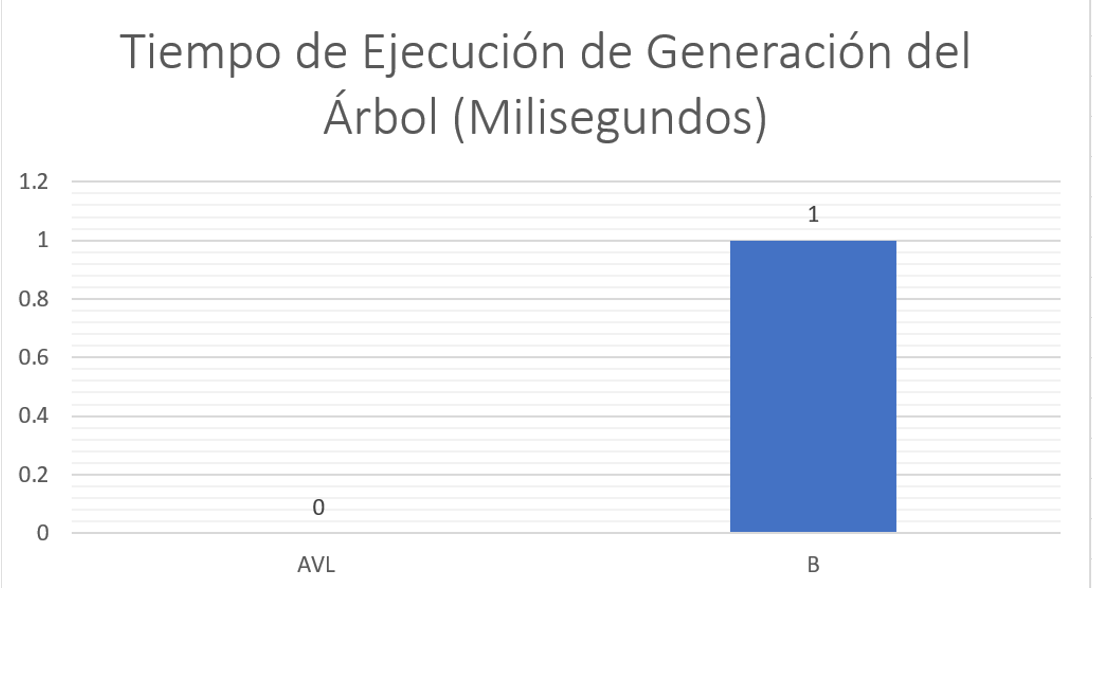
\includegraphics[angle=0,scale=0.6]{10.1 elem.png}
  
\end{figure}

\begin{figure}[h]
  \centering
  \caption{Gráfica Comparativa del Tiempo en la Búsqueda de 10 números en el Árbol de 10 elementos}

  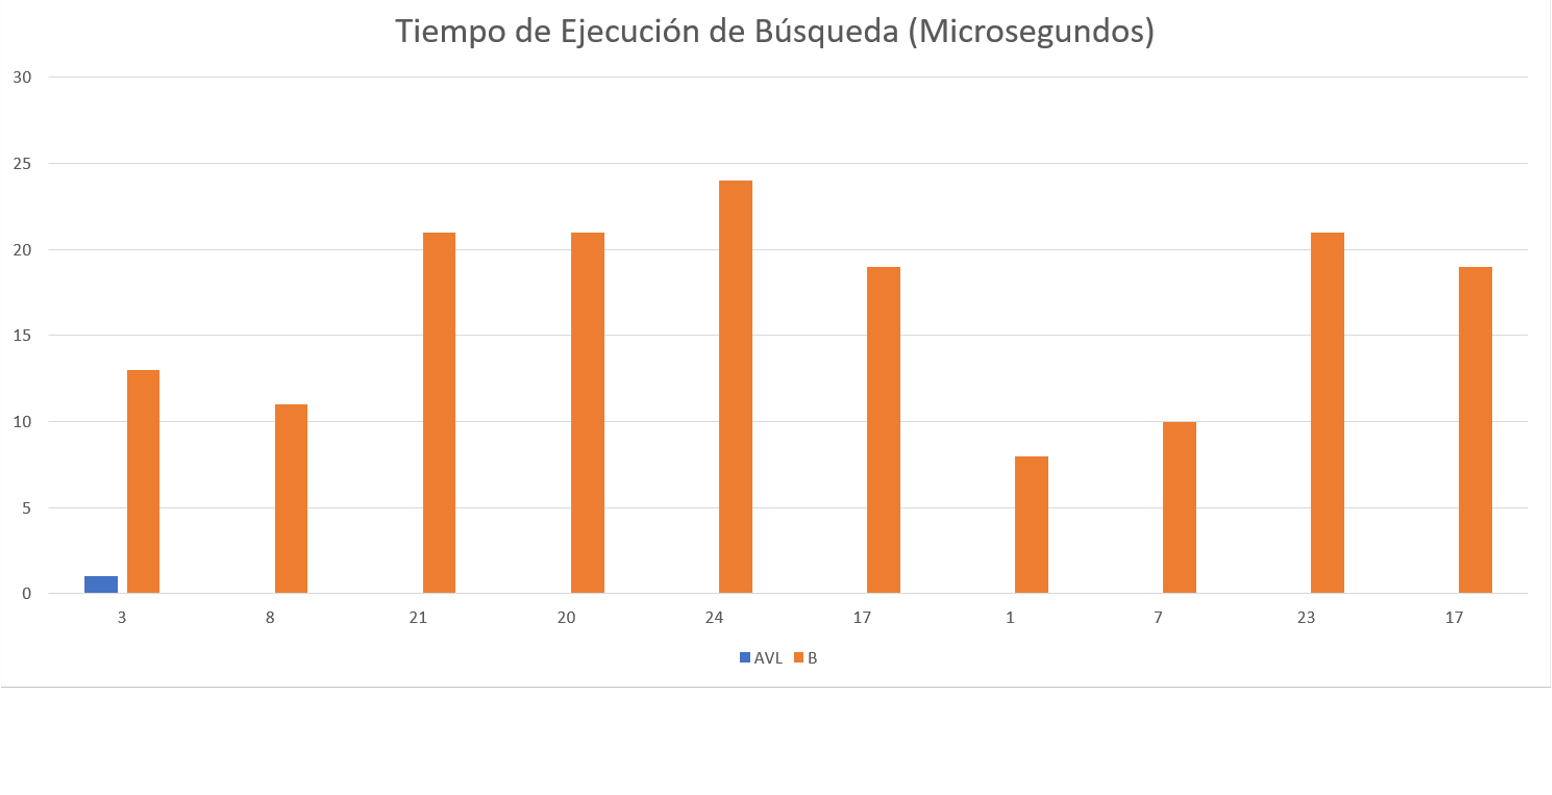
\includegraphics[angle=0,scale=0.5]{10.2 elem.png}
  
\end{figure}
\begin{figure}[h]
  \centering
  \caption{Gráfica Comparativa del Tiempo en la Eliminación de 10 números en el Árbol de 10 elementos}

  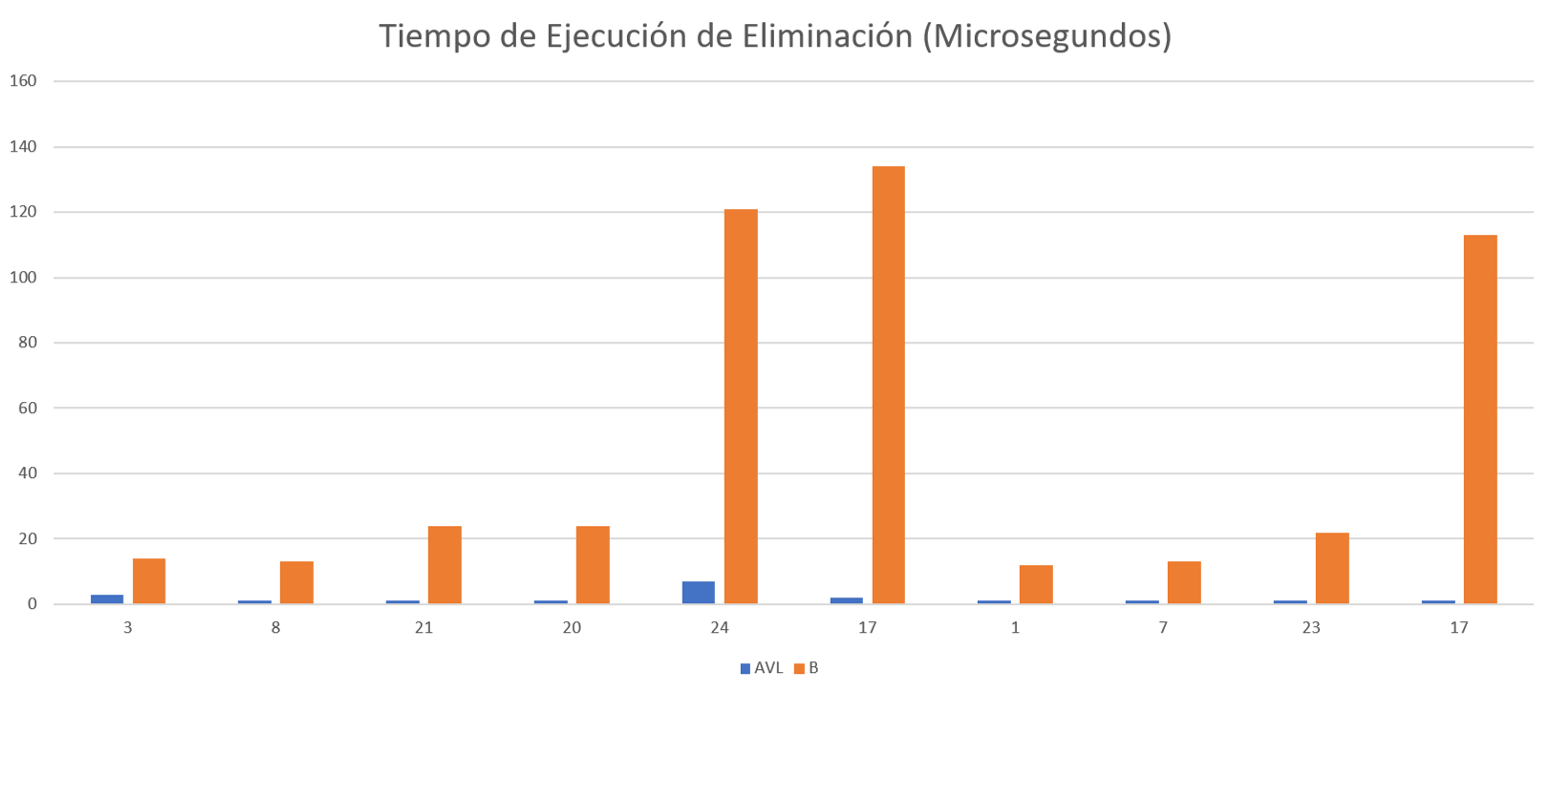
\includegraphics[angle=0,scale=0.5]{10.3 elem.png}
  
\end{figure}
\clearpage
%%------------------------------------------------


\begin{table}[htbp]
\begin{center}
  \caption{Inserción de 100 Elementos}
  \begin{tabular}{cc}
    \toprule
    AVL & B\\
    \midrule
    \texttt{0 milisegundos} & 20 milisegundos \\
    \bottomrule
  \end{tabular}
  \end{center}
\end{table}

\begin{table}[hbp]
\begin{center}
  \caption{Búsqueda de 10 Elementos en un Arbol de 100 Elementos}
  \begin{tabular}{ccccc}
    \toprule
    \multicolumn{5}{c}{BUSCAR}\\
    \midrule
     \, & AVL &\, & Arbol B & \,\\
     \, &Estado&Tiempo&Estado&Tiempo \\
      196 &ENCONTRADO&1 microseg&ENCONTRADO&35 microseg \\
      71 &NO ENCONTRADO&1 microseg&NO ENCONTRADO&34 microseg \\
      135 &ENCONTRADO&1 microseg&ENCONTRADO&47 microseg \\
      179 &NO ENCONTRADO&1 microseg&NO ENCONTRADO&48 microseg \\
      168 &NO ENCONTRADO&1 microseg&NO ENCONTRADO&39 microseg \\
      202 &NO ENCONTRADO&1 microseg&NO ENCONTRADO&35 microseg \\
      198 &NO ENCONTRADO&0 microseg&NO ENCONTRADO&33 microseg \\
      3 &NO ENCONTRADO&1 microseg&NO ENCONTRADO&28 microseg \\
       118 &NO ENCONTRADO&1 microseg&NO ENCONTRADO&43 microseg \\
      193 &ENCONTRADO&0 microseg&ENCONTRADO&11 microseg \\

    \bottomrule
  \end{tabular}
  \end{center}
\end{table}


\begin{table}[htbp]
\begin{center}
  \caption{Eliminación de 10 Elementos en un Arbol de 100 Elementos}
  \begin{tabular}{ccc}
    \toprule
    \multicolumn{3}{c}{Eliminar}\\
    \midrule
     Valor & AVL & Arbol B\\
      196 &20 microseg&633 microseg\\
      71 & 4 microseg&43 microseg\\
      135 &5 microseg &125 microseg\\
      179 &3 microseg&52 microseg\\
      168 & 3 microseg&41 microseg\\
      202 &3 microseg&46 microseg\\
      198 &3 microseg&46 microseg\\
      3 &3 microseg&28 microseg\\
       118 &3 microseg&42 microseg\\
      193 &4 microseg&125 microseg\\
    \bottomrule
  \end{tabular}
  \end{center}
\end{table}


\begin{figure}[hbp]
  \centering
  \caption{Gráfica Comparativa del Tiempo en la Generación del Árbol de 100 elementos}

  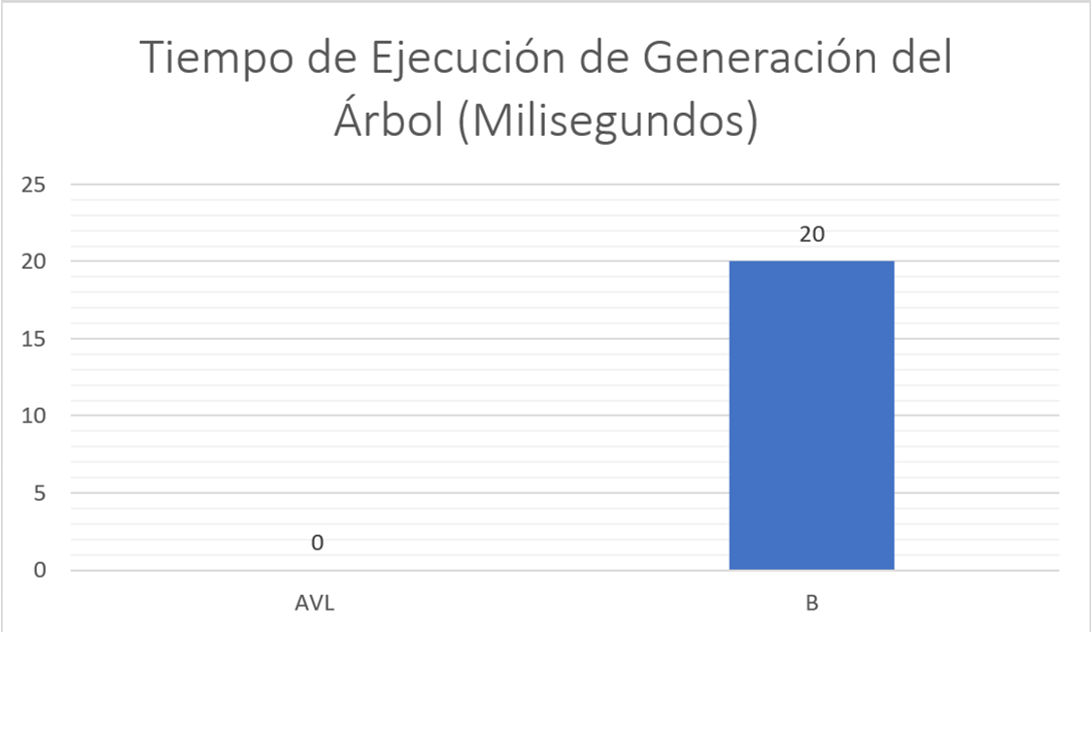
\includegraphics[angle=0,scale=0.6]{100.1 elem.png}
  
\end{figure}

\begin{figure}[hbp]
  \centering
  \caption{Gráfica Comparativa del Tiempo en la Búsqueda de 10 números en el Árbol de 100 elementos}

  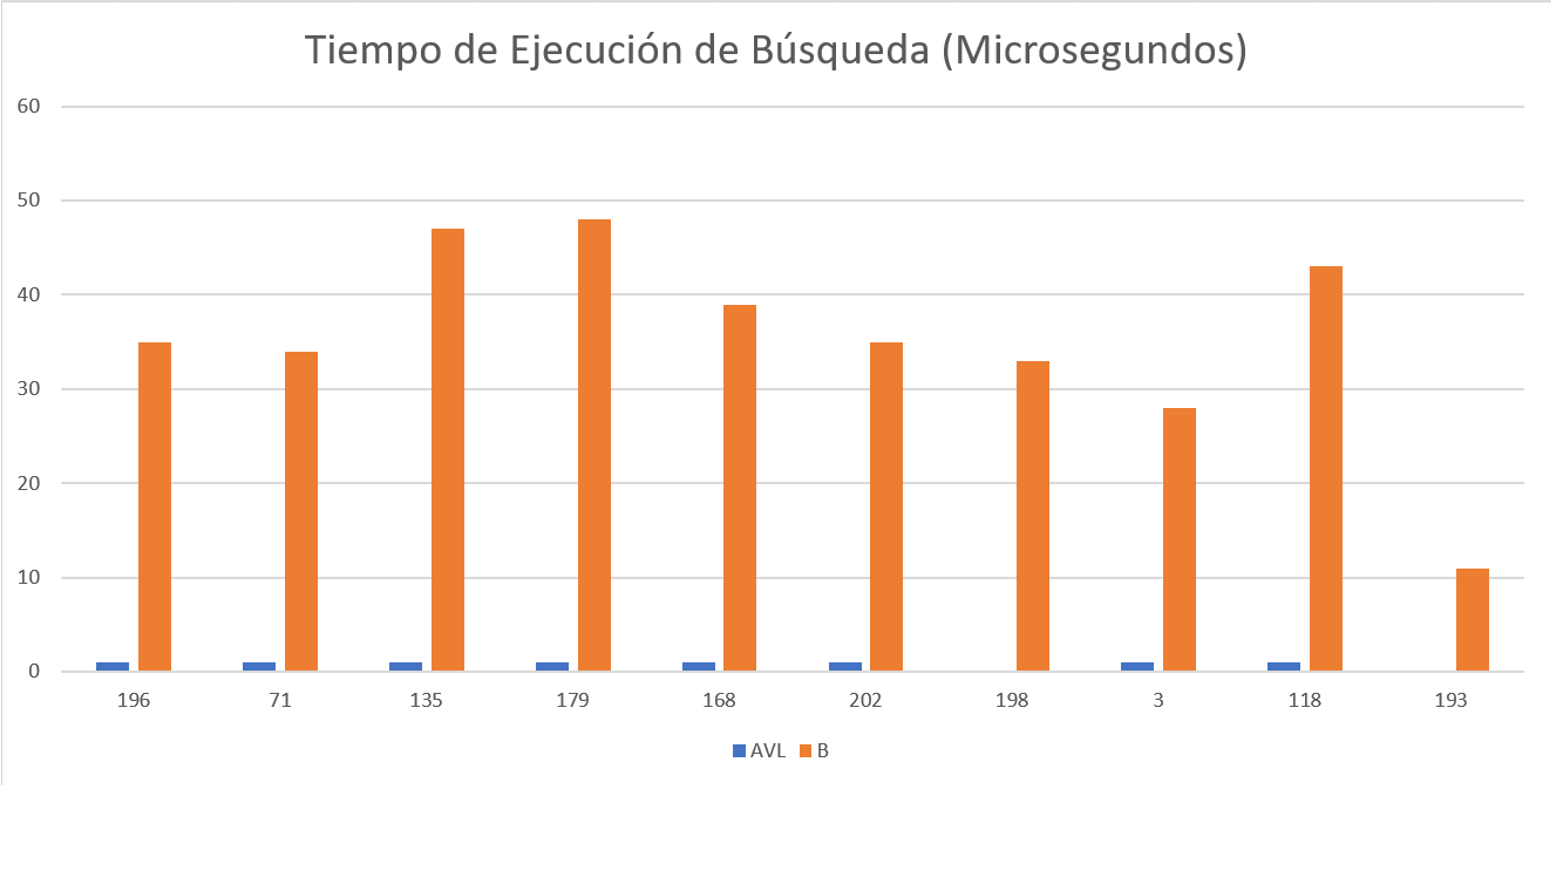
\includegraphics[angle=0,scale=0.5]{100.2 elem.png}
  
\end{figure}
\clearpage

\begin{figure}[h]
  \centering
  \caption{Gráfica Comparativa del Tiempo en la Eliminación de 10 números en el Árbol de 100 elementos}

  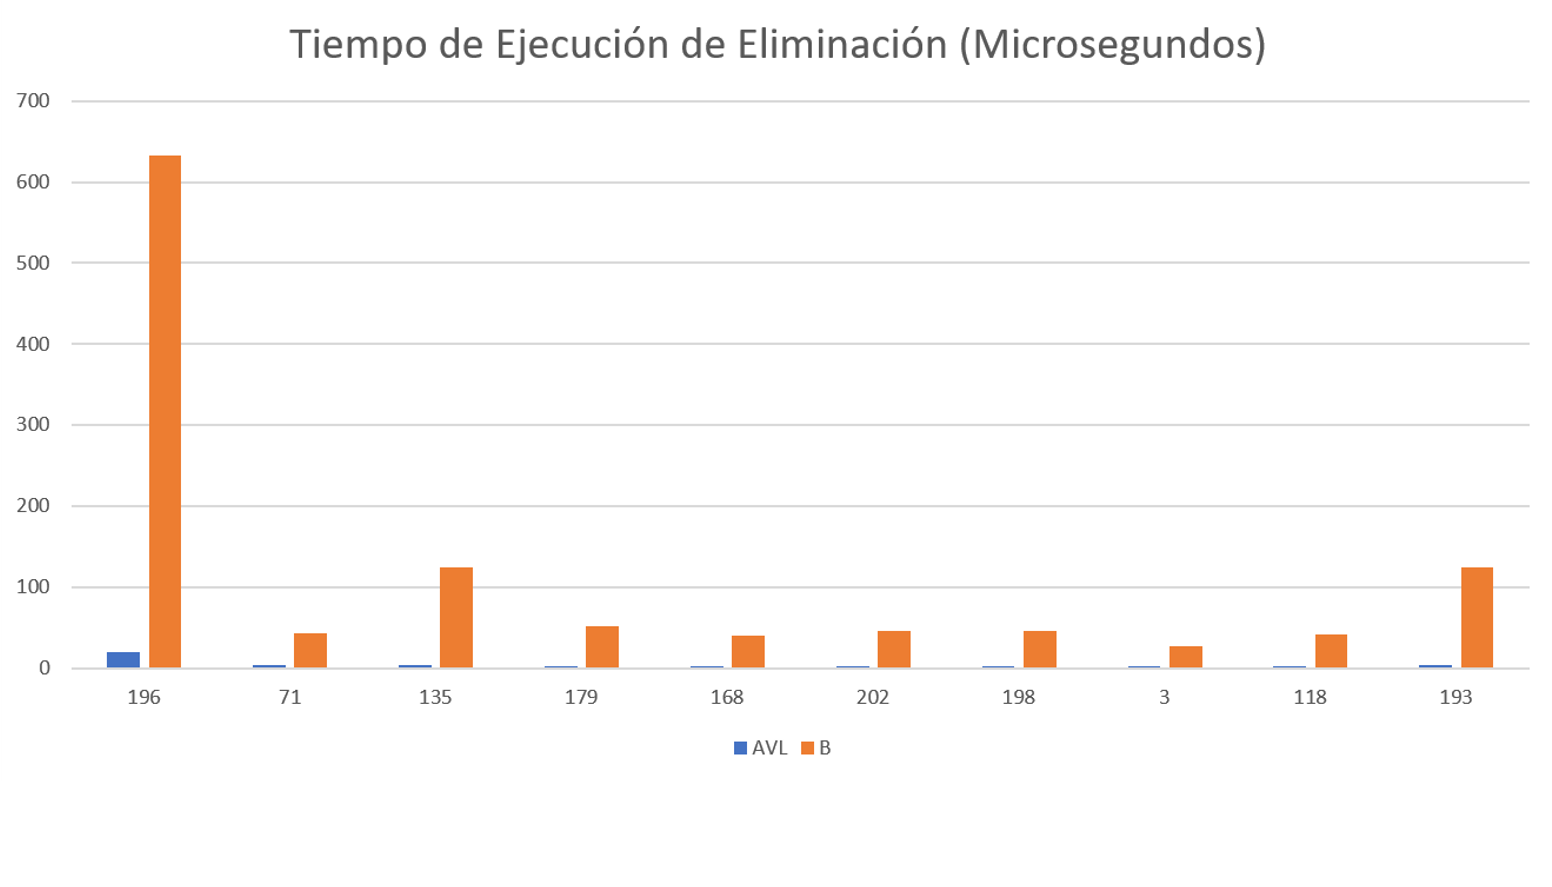
\includegraphics[angle=0,scale=0.5]{100.3 elem.png}
  
\end{figure}


%--------------------------------------------------------

\begin{table}[htbp]
\begin{center}
  \caption{Inserción de 1000 Elementos}
  \begin{tabular}{cc}
    \toprule
    AVL & B\\
    \midrule
    \texttt{3 milisegundos} & 260 milisegundos \\
    \bottomrule
  \end{tabular}
  \end{center}
\end{table}

\clearpage

\begin{table}[t]
\begin{center}
  \caption{Búsqueda de 10 Elementos en un Arbol de 1000 Elementos}
  \begin{tabular}{ccccc}
    \toprule
    \multicolumn{5}{c}{BUSCAR}\\
    \midrule
     \, & AVL &\, & Arbol B & \,\\
     \, &Estado&Tiempo&Estado&Tiempo \\
      2694 &NO ENCONTRADO&3 microseg&NO ENCONTRADO&83 microseg \\
      335 &NO ENCONTRADO&2 microseg&NO ENCONTRADO&76 microseg \\
      440 &NO ENCONTRADO&2 microseg&NO ENCONTRADO&68 microseg \\
      335 &NO ENCONTRADO&1 microseg&NO ENCONTRADO&81 microseg \\
      2422 & ENCONTRADO&1 microseg& ENCONTRADO&67 microseg \\
      2160 &NO ENCONTRADO&2 microseg&NO ENCONTRADO&65 microseg \\
      1986 &NO ENCONTRADO&2 microseg&NO ENCONTRADO&73 microseg \\
      958 &NO ENCONTRADO&2 microseg&NO ENCONTRADO&75 microseg \\
       2355 &NO ENCONTRADO&2 microseg&NO ENCONTRADO&71 microseg \\
      762 &ENCONTRADO&4 microseg&ENCONTRADO&98 microseg \\

    \bottomrule
  \end{tabular}
  \end{center}
\end{table}


\begin{table}[htbp]
\begin{center}
  \caption{Eliminación de 10 Elementos en un Arbol de 1000 Elementos}
  \begin{tabular}{ccc}
    \toprule
    \multicolumn{3}{c}{Eliminar}\\
    \midrule
     Valor & AVL & Arbol B\\
     2694 &8 microseg&623 microseg \\
      335 &5 microseg&600 microseg \\
      440 &5 microseg&121 microseg \\
      335 &4 microseg&149 microseg \\
      2422 &20 microseg& 743 microseg \\
      2160 &5 microseg&80 microseg \\
      1986 &5 microseg&123 microseg \\
      958 &5 microseg&583 microseg \\
       2355 &5 microseg&558 microseg \\
      762 &5 microseg&204 microseg \\


    \bottomrule
  \end{tabular}
  \end{center}
\end{table}
\clearpage

\begin{figure}[htbp]
  \centering
  \caption{Gráfica Comparativa del Tiempo en la Generación del Árbol de 1000 elementos}

  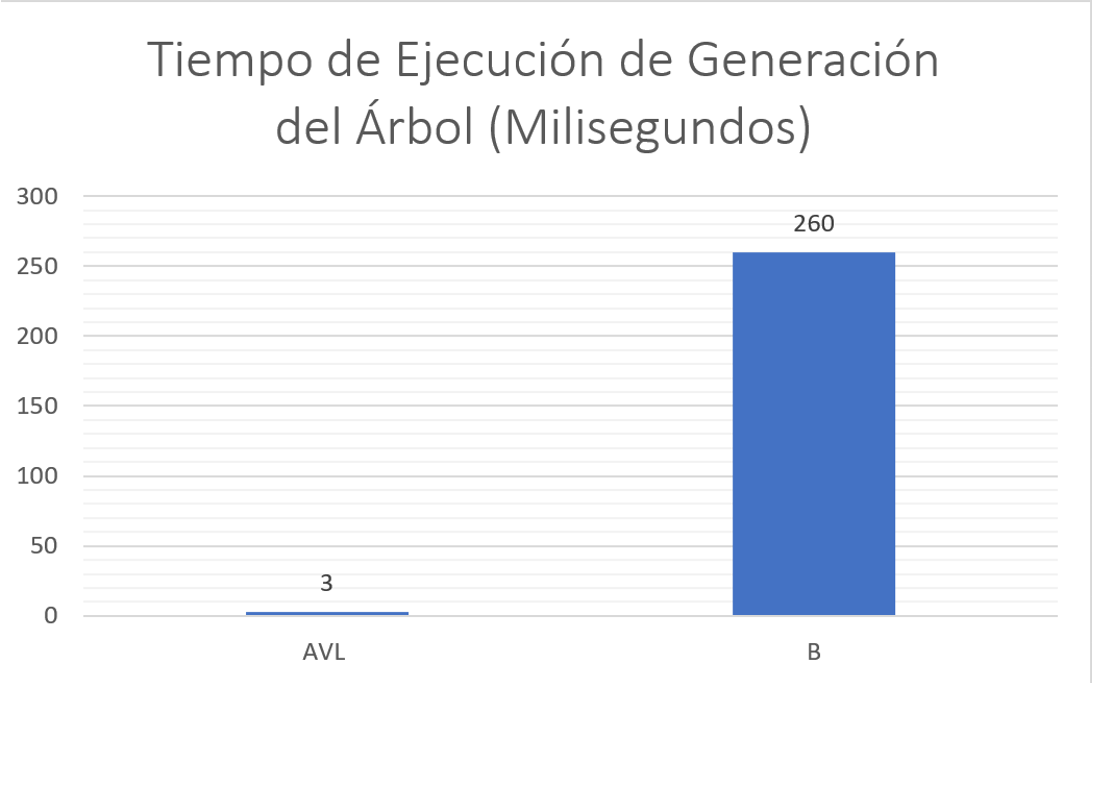
\includegraphics[angle=0,scale=0.6]{1000.1 elem.png}
  
\end{figure}
\begin{figure}[hp]
  \centering
  \caption{Gráfica Comparativa del Tiempo en la Búsqueda de 10 números en el Árbol de 1000 elementos}

  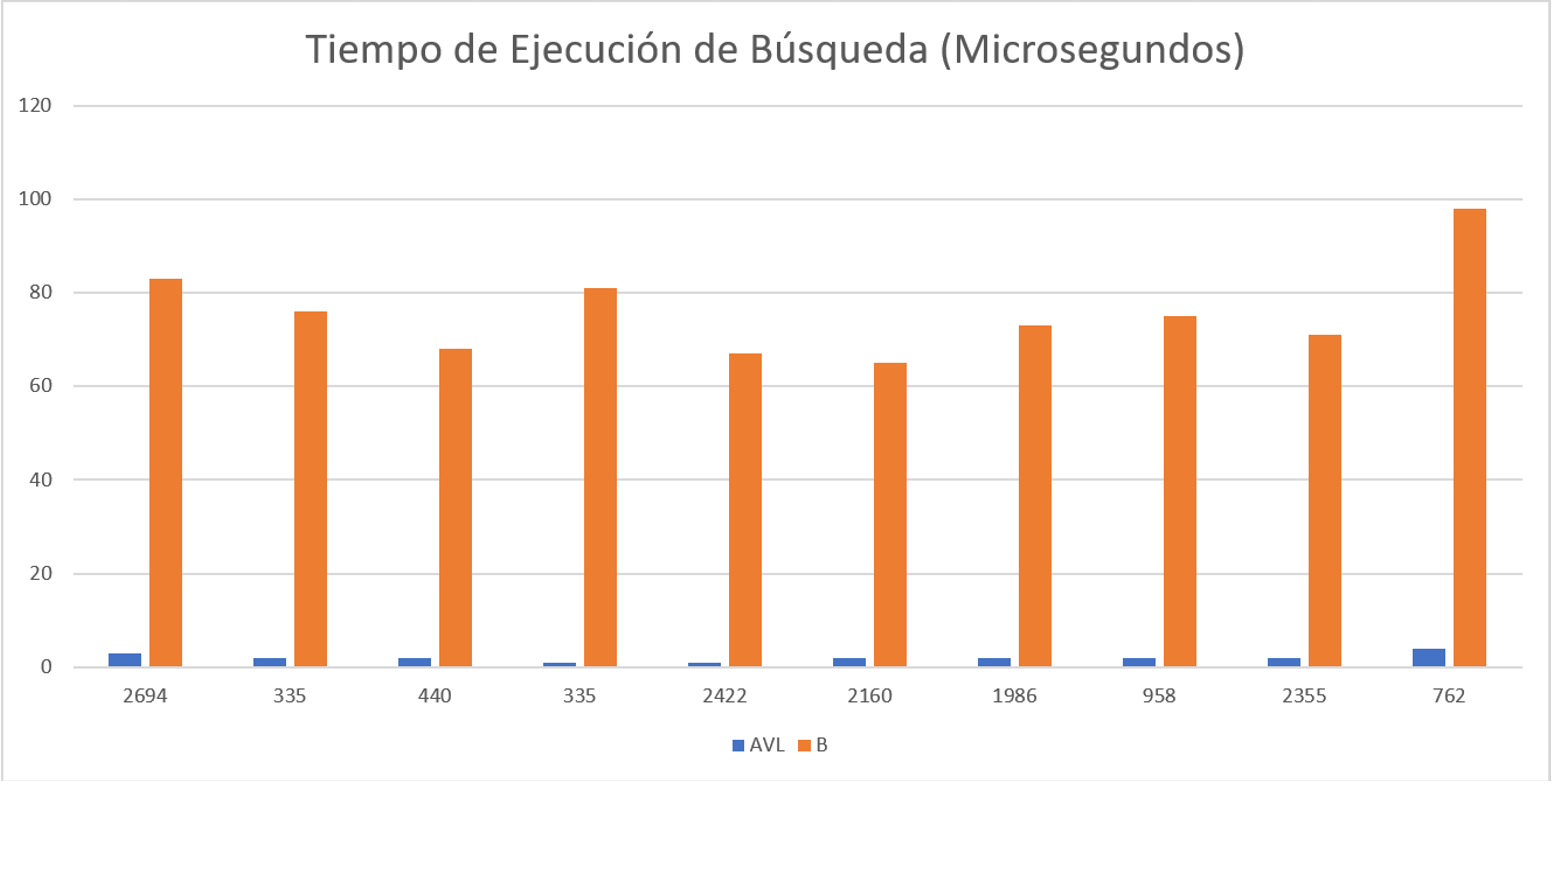
\includegraphics[angle=0,scale=0.5]{1000.2 elem.png}
  
\end{figure}

\begin{figure}[ht]
  \centering
  \caption{Gráfica Comparativa del Tiempo en la Eliminación de 10 números en el Árbol de 1000 elementos}

  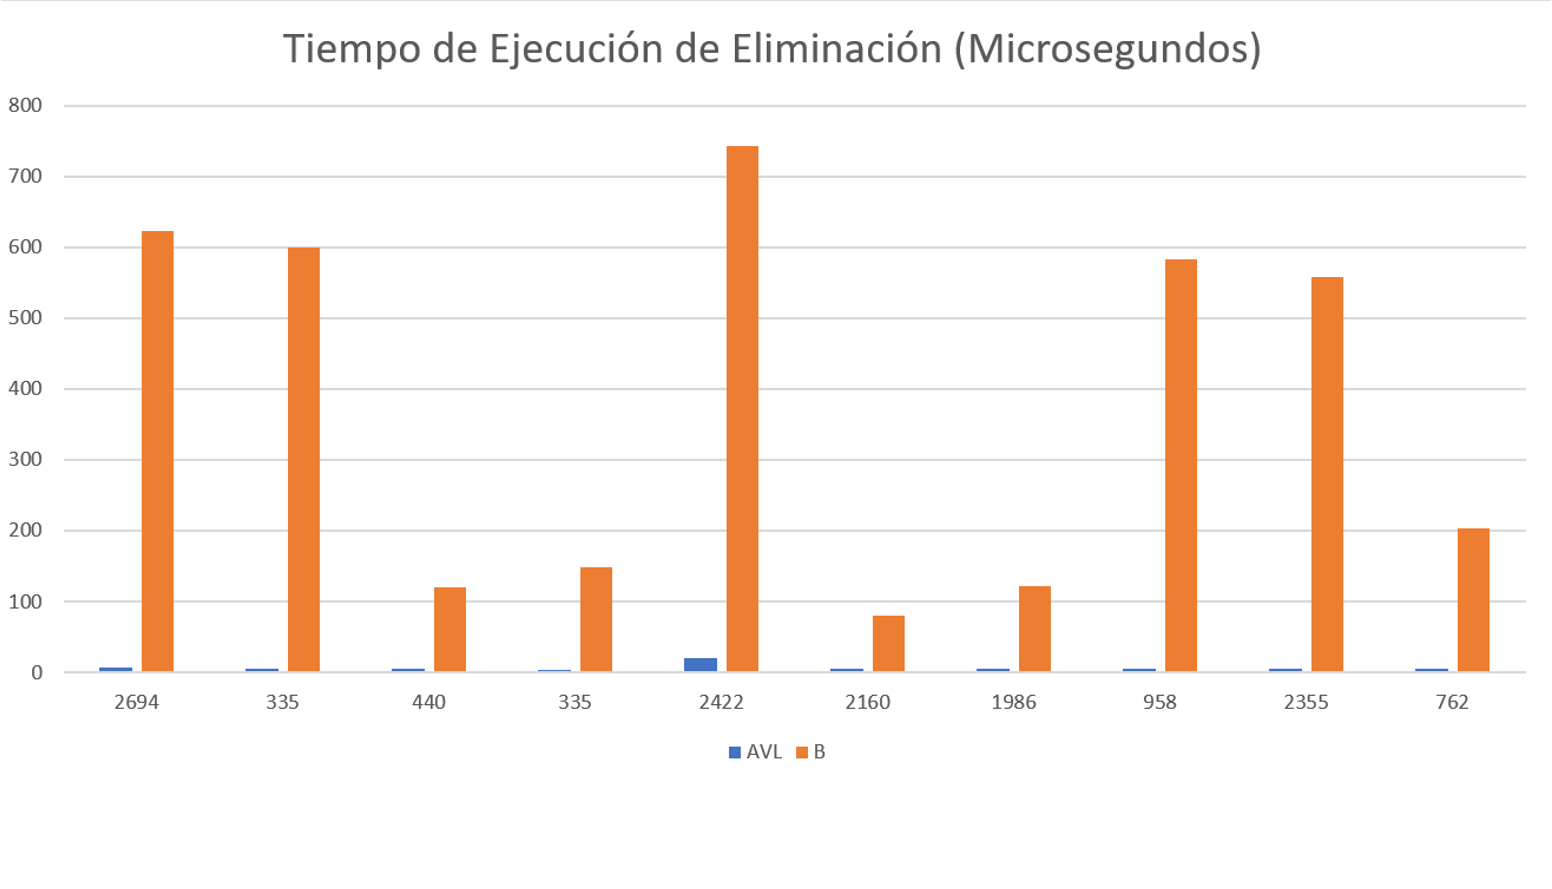
\includegraphics[angle=0,scale=0.5]{1000.3 elem.png}
  
\end{figure}


%--------------------------------------------------
\begin{table}[htbp]
\begin{center}
  \caption{Inserción de 10000 Elementos}
  \begin{tabular}{cc}
    \toprule
    AVL & B\\
    \midrule
    \texttt{52 milisegundos} & 3319 milisegundos \\
    \bottomrule
  \end{tabular}
  \end{center}
\end{table}
\clearpage
\begin{table}[htbp]
\begin{center}
  \caption{Búsqueda de 10 Elementos en un Arbol de 10000 Elementos}
  \begin{tabular}{ccccc}
    \toprule
    \multicolumn{5}{c}{BUSCAR}\\
    \midrule
     \, & AVL &\, & Arbol B & \,\\
     \, &Estado&Tiempo&Estado&Tiempo \\
     
      17538 &ENCONTRADO&4 microseg&ENCONTRADO&112 microseg \\
      28411 &NO ENCONTRADO&3 microseg&NO ENCONTRADO&124 microseg \\
      3757 &NO ENCONTRADO&4 microseg&NO ENCONTRADO&107 microseg \\
      17668 &ENCONTRADO&2 microseg&ENCONTRADO&77 microseg \\
      25313 &NO ENCONTRADO&5 microseg&NO ENCONTRADO&121 microseg \\
      12063 &NO ENCONTRADO&5 microseg&NO ENCONTRADO&121 microseg \\
      14137 &NO ENCONTRADO&2 microseg&NO ENCONTRADO&105 microseg \\
      7230 &NO ENCONTRADO&4 microseg&NO ENCONTRADO&101 microseg \\
       6847 &NO ENCONTRADO&2 microseg&NO ENCONTRADO&126 microseg \\
      9903 &NO ENCONTRADO&2 microseg&NO ENCONTRADO&119 microseg \\

    \bottomrule
  \end{tabular}
  \end{center}
\end{table}


\begin{table}[htbp]
\begin{center}
  \caption{Eliminación de 10 Elementos en un Arbol de 10000 Elementos}
  \begin{tabular}{ccc}
    \toprule
    \multicolumn{3}{c}{Eliminar}\\
    \midrule
     Valor & AVL & Arbol B\\
      17538 &24 microseg&751 microseg \\
      28411 &7 microseg&192 microseg \\
      3757 &8 microseg&955 microseg \\
      17668 &9 microseg&763 microseg \\
      25313 &9 microseg&191 microseg \\
      12063 &8 microseg&7878 microseg \\
      14137 &10 microseg&1259 microseg \\
      7230 &11 microseg&191 microseg \\
       6847 &8 microseg&175 microseg \\
      9903 &8 microseg&203 microseg \\

    \bottomrule
  \end{tabular}
  \end{center}
\end{table}
\clearpage

\begin{figure}[hbp]
  \centering
  \caption{Gráfica Comparativa del Tiempo en la Generación del Árbol de 10000 elementos}

  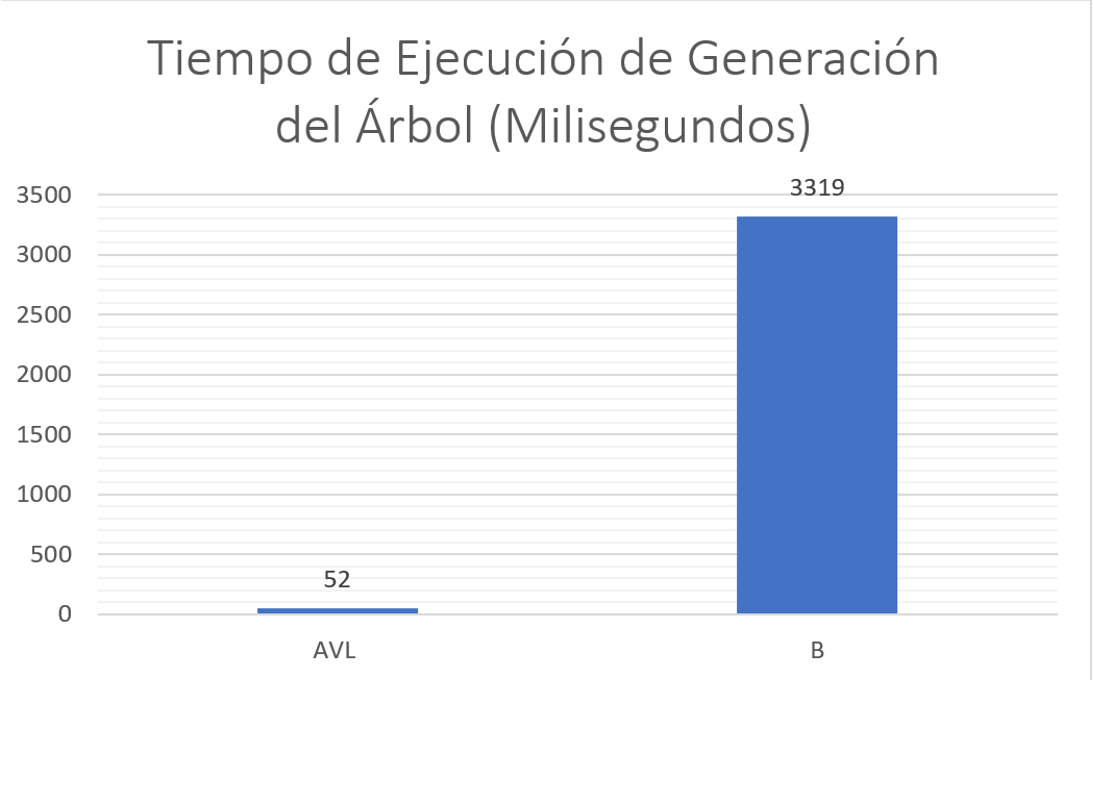
\includegraphics[angle=0,scale=0.6]{10000.1 elem.png}
  
\end{figure}
\begin{figure}[hbp]
  \centering
  \caption{Gráfica Comparativa del Tiempo en la Búsqueda de 10 números en el Árbol de 10000 elementos}

  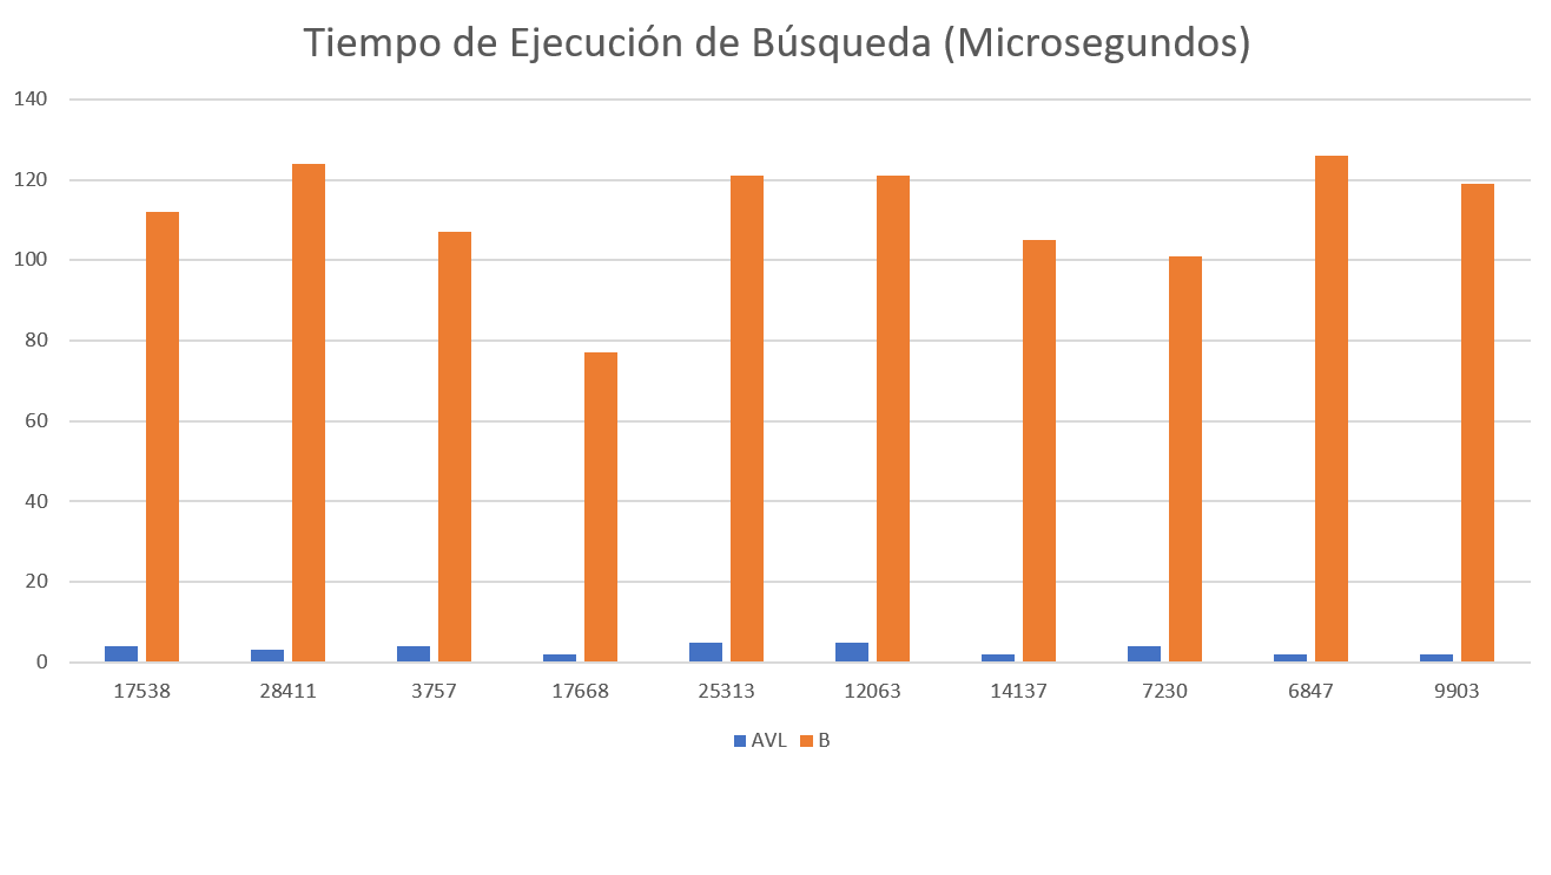
\includegraphics[angle=0,scale=0.5]{10000.2 elem.png}
  
\end{figure}
\begin{figure}[ht]
  \centering
  \caption{Gráfica Comparativa del Tiempo en la Eliminación de 10 números en el Árbol de 10000 elementos}

  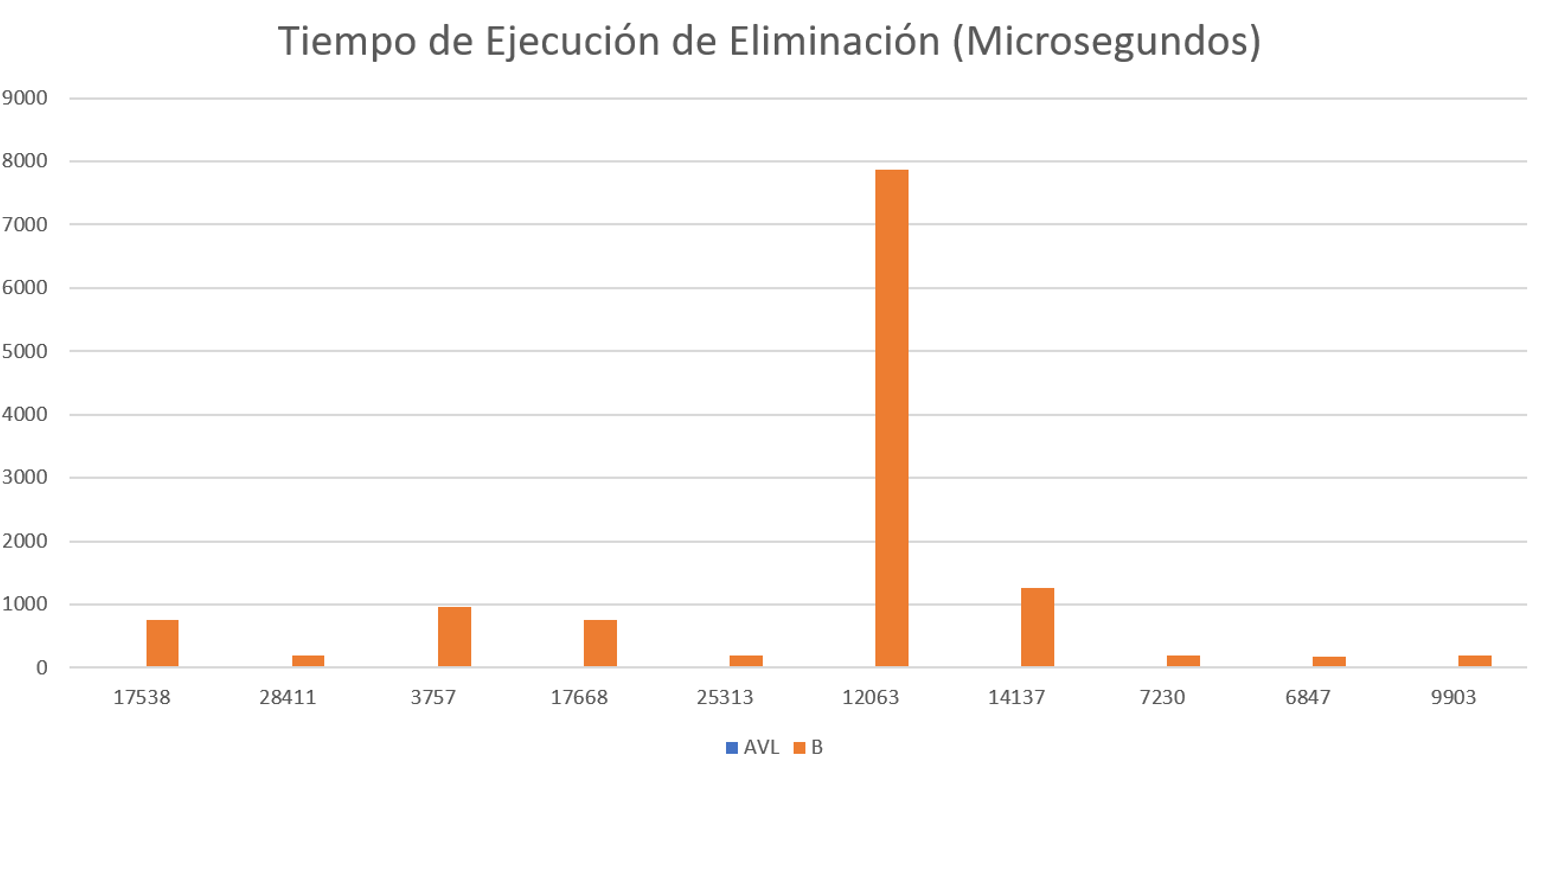
\includegraphics[angle=0,scale=0.5]{10000.3 elem.png}
  
\end{figure}
%----------------------------------------------------------------------


\begin{table}[htbp]
\begin{center}
  \caption{Inserción de 100000 Elementos}
  \begin{tabular}{cc}
    \toprule
    AVL & B\\
    \midrule
    \texttt{769 milisegundos} & 40407 milisegundos \\
    \bottomrule
  \end{tabular}
  \end{center}
\end{table}

\begin{table}[htbp]
\begin{center}
  \caption{Búsqueda de 10 Elementos en un Arbol de 100000 Elementos}
  \begin{tabular}{ccccc}
    \toprule
    \multicolumn{5}{c}{BUSCAR}\\
    \midrule
     \, & AVL &\, & Arbol B & \,\\
     \, &Estado&Tiempo&Estado&Tiempo \\
     
      112643 &ENCONTRADO&6 microseg&ENCONTRADO&194 microseg \\
      110719 &NO ENCONTRADO&4 microseg&NO ENCONTRADO&170 microseg \\
      266017 &ENCONTRADO&3 microseg& ENCONTRADO&133 microseg \\
      80717 &NO ENCONTRADO&5 microseg&NO ENCONTRADO&161 microseg \\
      208264 &NO ENCONTRADO&7 microseg&NO ENCONTRADO&169 microseg \\
      162107 &NO ENCONTRADO&5 microseg&NO ENCONTRADO&134 microseg \\
      189429 &NO ENCONTRADO&4 microseg&NO ENCONTRADO&124 microseg \\
      99767 &ENCONTRADO&6 microseg&ENCONTRADO&162 microseg \\
       16840 &NO ENCONTRADO&4 microseg&NO ENCONTRADO&120 microseg \\
      138042 &ENCONTRADO&4 microseg&ENCONTRADO&171 microseg \\

    \bottomrule
  \end{tabular}
  \end{center}
\end{table}

\begin{table}[htbp]
\begin{center}
  \caption{Eliminación de 10 Elementos en un Arbol de 100000 Elementos}
  \begin{tabular}{ccc}
    \toprule
    \multicolumn{3}{c}{Eliminar}\\
    \midrule
     Valor & AVL & Arbol B\\
      112643 &26 microseg&1389 microseg \\
      110719 &12 microseg&829 microseg \\
      266017 &15 microseg&1224 microseg \\
      80717 &12 microseg&1195 microseg \\
      208264 &11 microseg&761 microseg \\
      162107 &12 microseg&5358 microseg \\
      189429 &15 microseg&225 microseg \\
      99767 &14 microseg&1948 microseg \\
       16840 &14 microseg&1654 microseg \\
      138042 &15 microseg&1440 microseg \\


    \bottomrule
  \end{tabular}
  \end{center}
\end{table}


\begin{figure}[ht]
  \centering
  \caption{Gráfica Comparativa del Tiempo en la Generación del Árbol de 100000 elementos}

  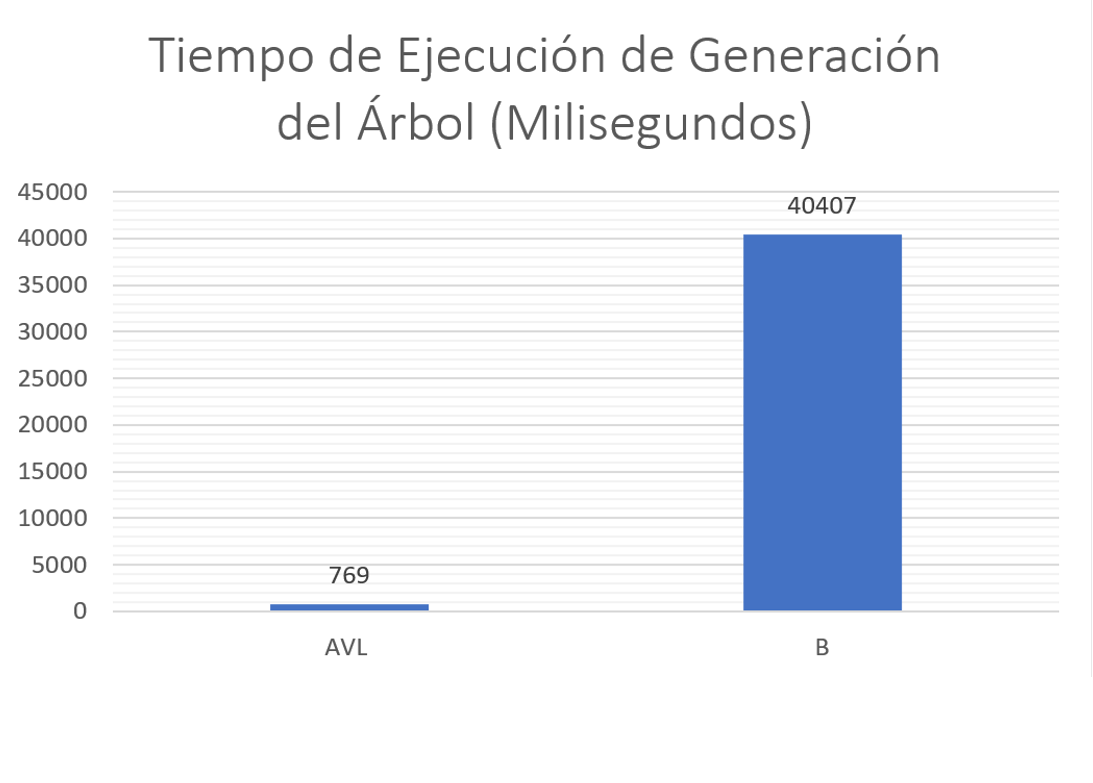
\includegraphics[angle=0,scale=0.6]{100000.1 elem.png}
  
\end{figure}
\begin{figure}[ht]
  \centering
  \caption{Gráfica Comparativa del Tiempo en la Búsqueda de 10 números en el Árbol de 100000 elementos}

  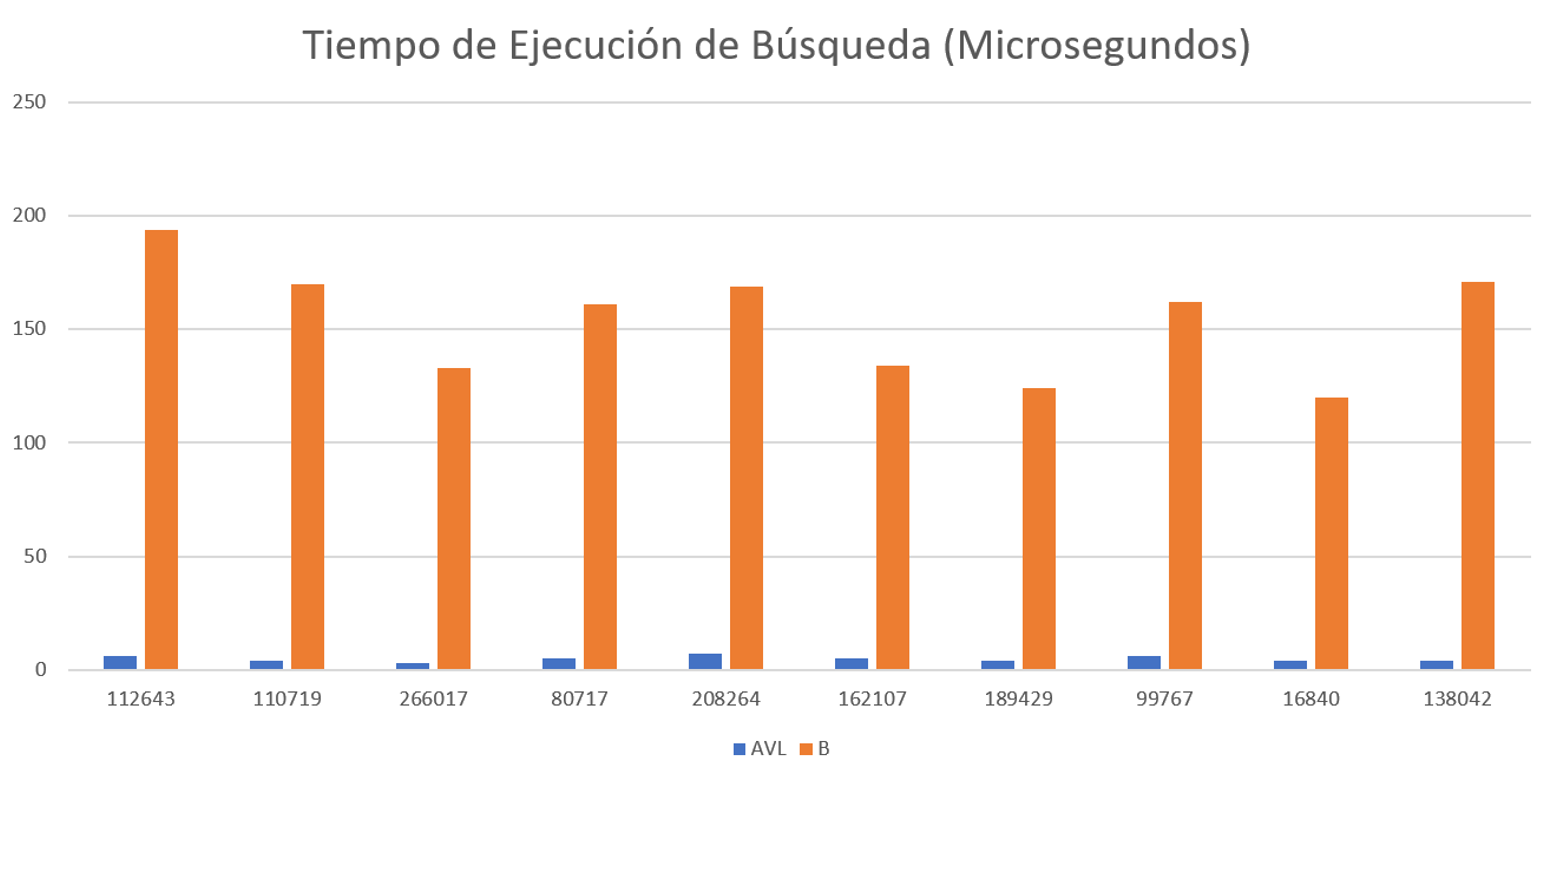
\includegraphics[angle=0,scale=0.53]{100000.2 elem.png}
  
\end{figure}

\begin{figure}[ht]
  \centering
  \caption{Gráfica Comparativa del Tiempo en la Eliminación de 10 números en el Árbol de 100000 elementos}

  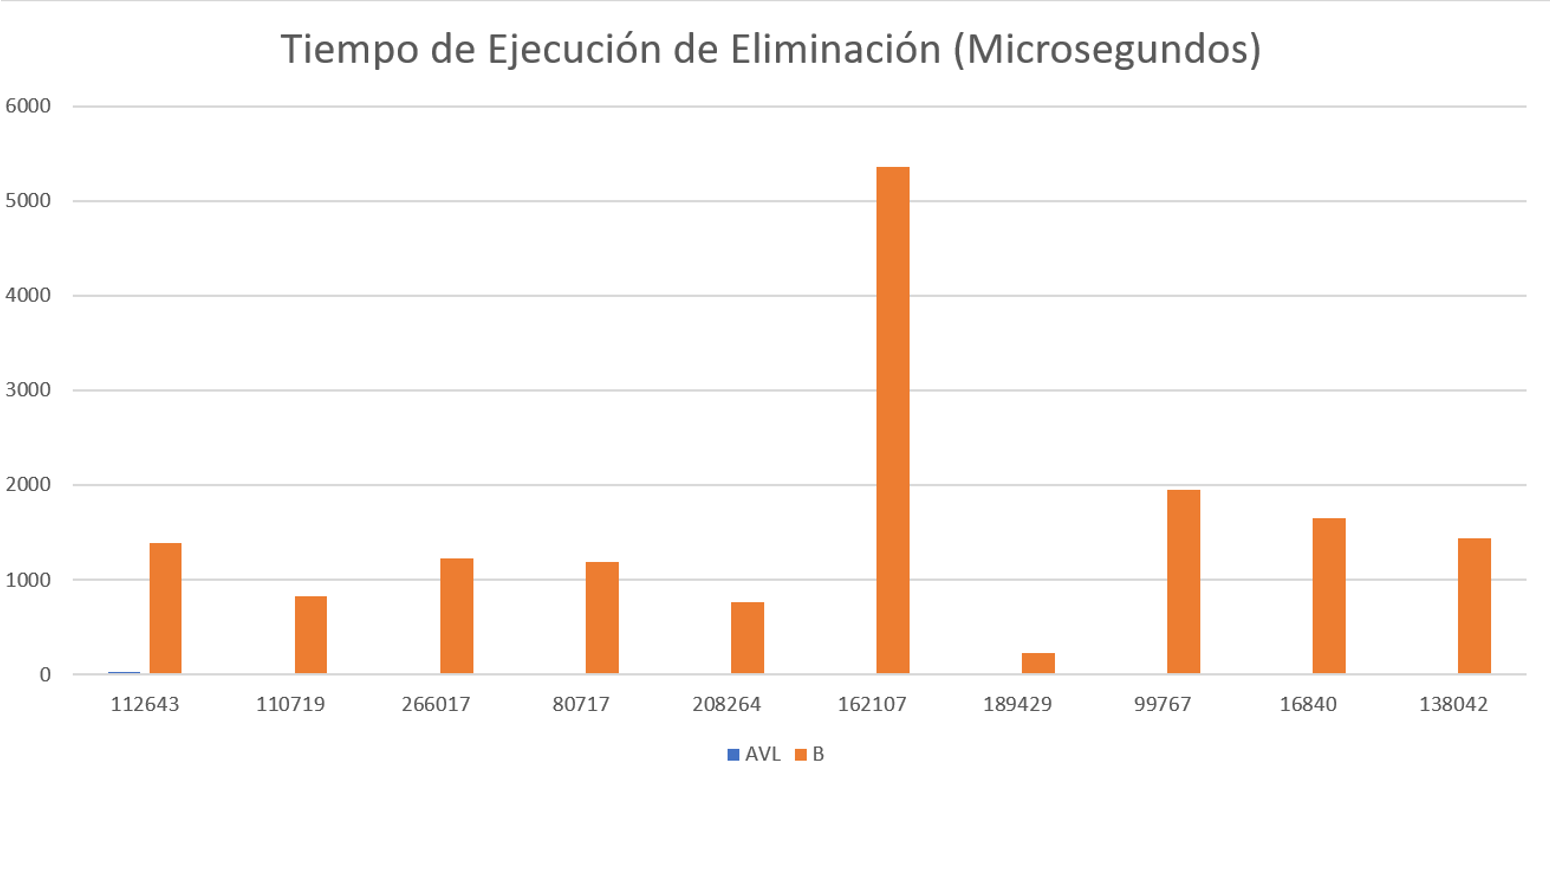
\includegraphics[angle=0,scale=0.5]{100000.3 elem.png}
  
\end{figure}

\clearpage

%----------------------------------------------------------------------


\begin{table}[t]
\begin{center}
  \caption{Inserción de 1000000 Elementos}
  \begin{tabular}{cc}
    \toprule
    AVL & B\\
    \midrule
    \texttt{11196 milisegundos} & 580190 milisegundos \\
    \bottomrule
  \end{tabular}
  \end{center}
\end{table}

\begin{table}[H]
\begin{center}
  \caption{Búsqueda de 10 Elementos en un Arbol de 1000000 Elementos}
  \begin{tabular}{ccccc}
    \toprule
    \multicolumn{5}{c}{BUSCAR}\\
    \midrule
     \, & AVL &\, & Arbol B & \,\\
     \, &Estado&Tiempo&Estado&Tiempo \\
  126690&NO ENCONTRADO&8 microseg&NO ENCONTRADO&145 microseg\\ 
  2371364&ENCONTRADO&7 microseg&ENCONTRADO&158 microseg\\
  946885&NO ENCONTRADO&7 microseg&NO ENCONTRADO&154 microseg\\
  848594&NO ENCONTRADO&7 microseg &NO ENCONTRADO&164 microseg\\ 
  2139382&NO ENCONTRADO&6 microseg&NO ENCONTRADO&155 microseg\\
  681756&ENCONTRADO&5 microseg&ENCONTRADO&284 microseg\\
  572207&NO ENCONTRADO&5 microseg&NO ENCONTRADO&231 microseg\\
  1790994&NO ENCONTRADO&8 microseg &NO ENCONTRADO&183 microseg\\
  739962&NO ENCONTRADO&6 microseg&NO ENCONTRADO&126 microseg\\
  214751&NO ENCONTRADO&7 microseg&NO ENCONTRADO&157 microseg\\

    \bottomrule
  \end{tabular}
  \end{center}
\end{table}


\begin{table}[htbp]
\begin{center}
  \caption{Eliminación de 10 Elementos en un Arbol de 1000000 Elementos}
  \begin{tabular}{ccc}
    \toprule
    \multicolumn{3}{c}{Eliminar}\\
    \midrule
     Valor & AVL & Arbol B\\
126690&16 microseg&2387 microseg\\

2371364&35 microseg&2564 microseg\\ 

946885&19 microseg&1847 microseg\\

848594&17 microseg&2241 microseg\\

2139382&18 microseg&2783 microseg\\

681756&21 microseg&444 microseg\\

572207&17 microseg&309 microseg\\

1790994&17 microseg&1854 microseg\\

739962&16 microseg&212 microseg\\

214751&15 microseg&1196 microseg\\


    \bottomrule
  \end{tabular}
  \end{center}
\end{table}

\clearpage
\begin{figure}[ht]
  \centering
  \caption{Gráfica Comparativa del Tiempo en la Generación del Árbol de 1000000 elementos}

  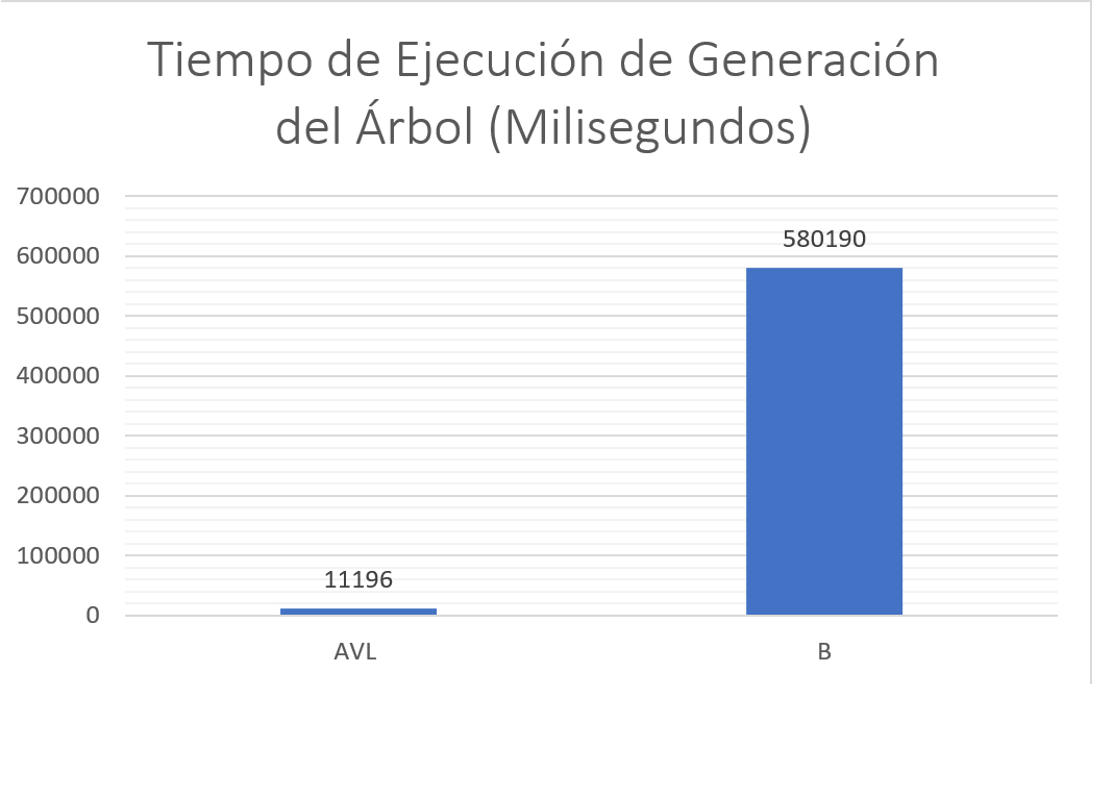
\includegraphics[angle=0,scale=0.6]{1000000.1 elem.png}
  
\end{figure}
\begin{figure}[ht]
  \centering
  \caption{Gráfica Comparativa del Tiempo en la Búsqueda de 10 números en el Árbol de 1000000 elementos}

  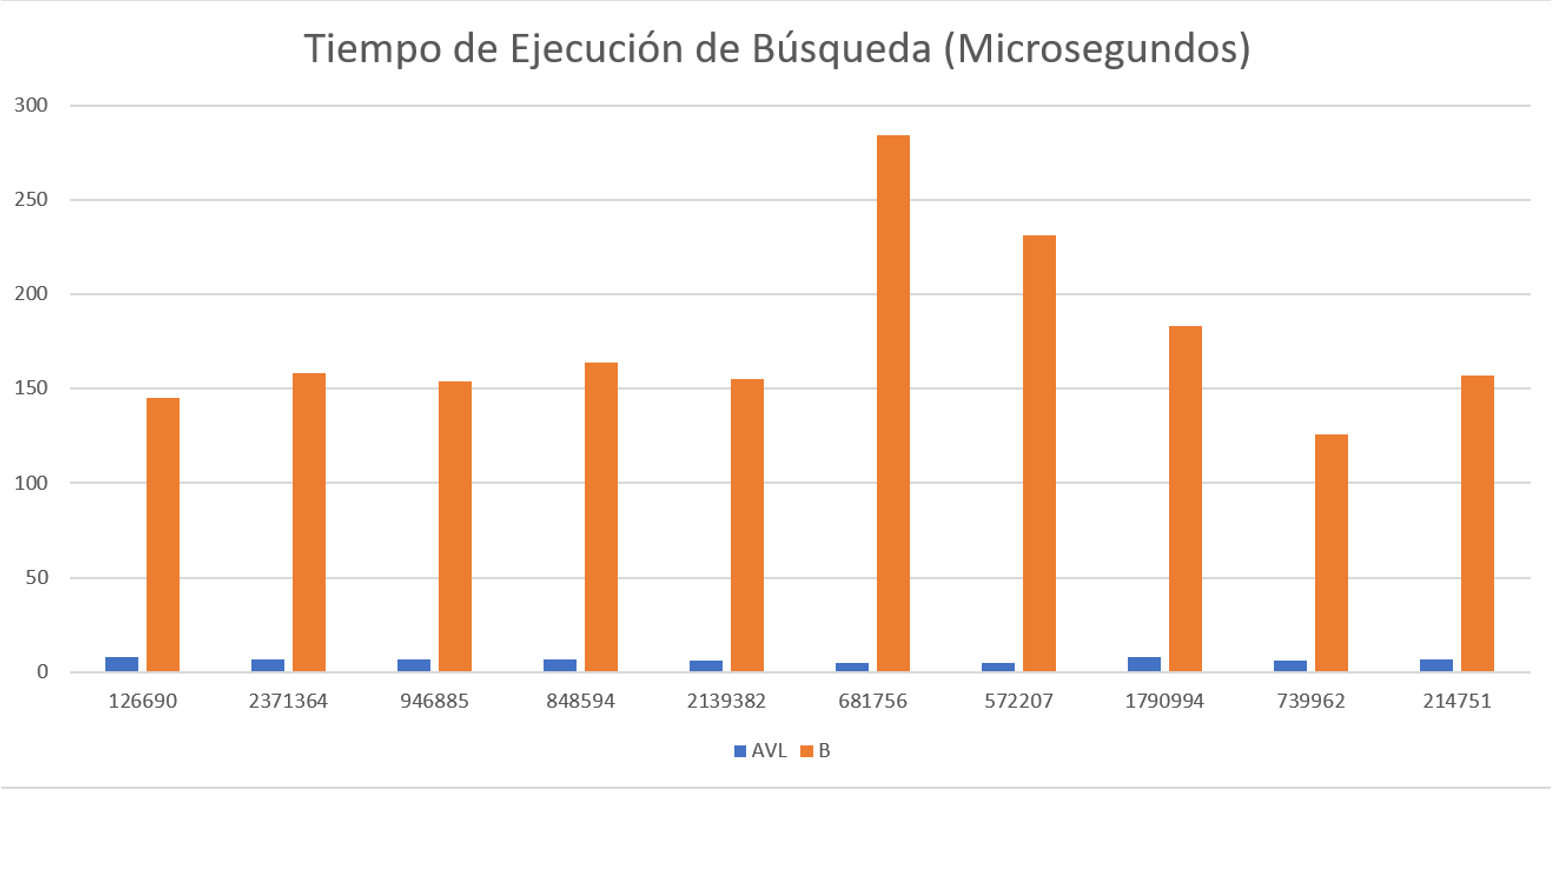
\includegraphics[angle=0,scale=0.53]{1000000.2 elem.png}
  
\end{figure}

\begin{figure}[ht]
  \centering
  \caption{Gráfica Comparativa del Tiempo en la Eliminación de 10 números en el Árbol de 1000000 elementos}

  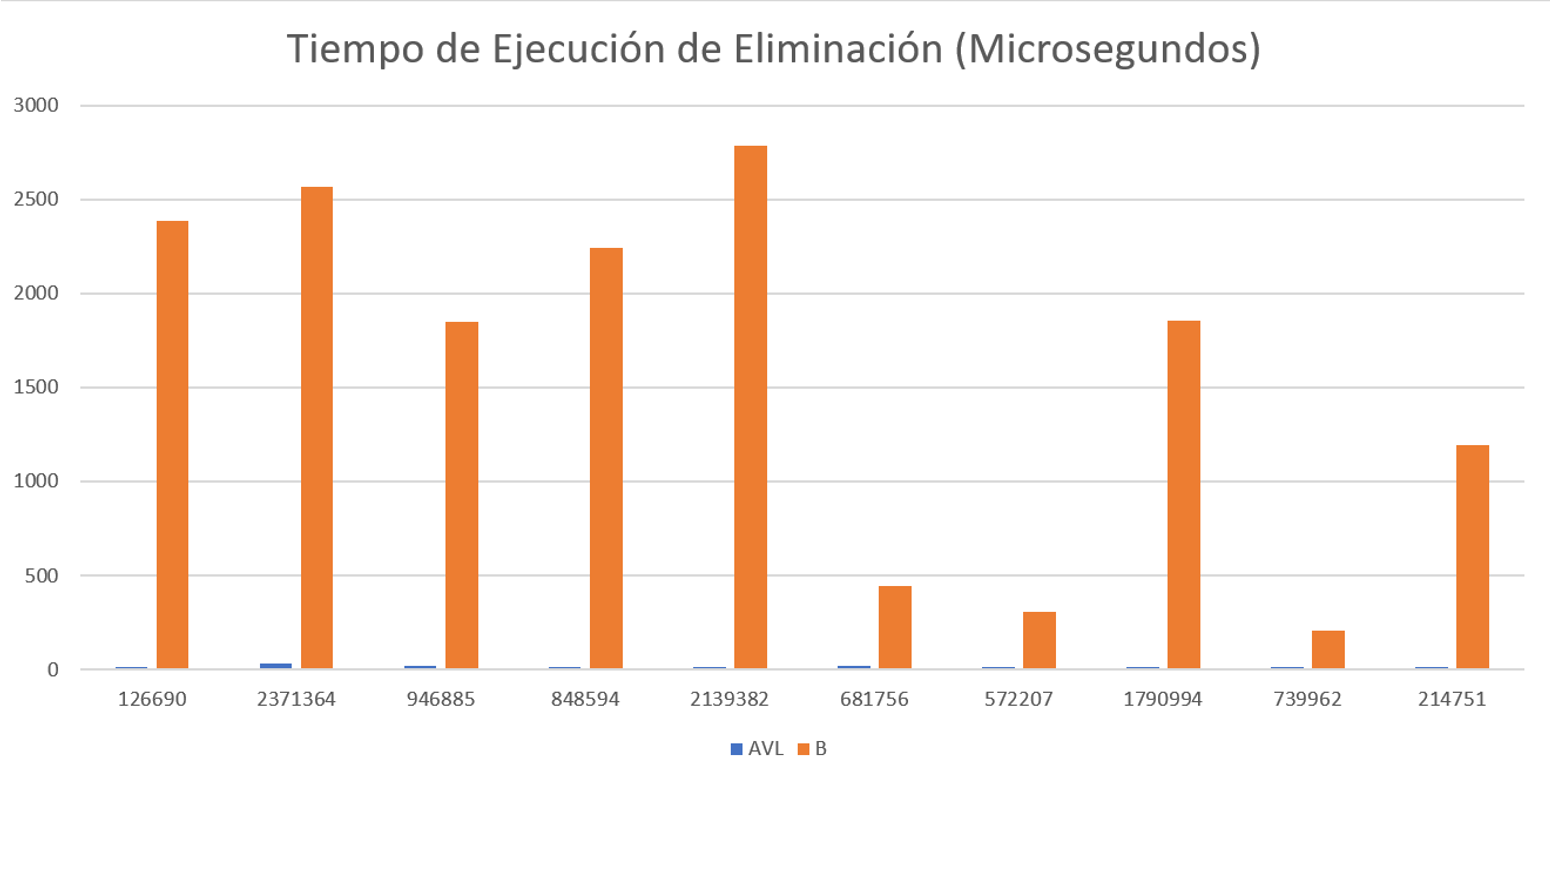
\includegraphics[angle=0,scale=0.5]{1000000.3 elem.png}
  
\end{figure}


%-------------------------------------------------------


\begin{table}[htbp]
\begin{center}
  \caption{Inserción de 2000000 Elementos}
  \begin{tabular}{cc}
    \toprule
    AVL & B\\
    \midrule
    \texttt{25850 milisegundos} & 1674505 milisegundos \\
    \bottomrule
  \end{tabular}
  \end{center}
\end{table}

\begin{table}[htbp]
\begin{center}
  \caption{Búsqueda de 10 Elementos en un Arbol de 2000000 Elementos}
  \begin{tabular}{ccccc}
    \toprule
    \multicolumn{5}{c}{BUSCAR}\\
    \midrule
     \, & AVL &\, & Arbol B & \,\\
     \, &Estado&Tiempo&Estado&Tiempo \\
     
4087517&ENCONTRADO&8 microseg&ENCONTRADO&159 microseg\\

2898064&ECONTRADO&9 microseg&ENCONTRADO&261 microseg\\

34929&NO ENCONTRADO&8 microseg&NO ENCONTRADO&170 microseg\\

887923&ENCONTRADO&8 microseg&ENCONTRADO&259 microseg\\

451742&ENCONTRADO&5 microseg&ENCONTRADO&147 microseg\\

2038671&NO ENCONTRADO&7 microseg&NO ENCONTRADO&269 microseg\\

209449&ENCONTRADO&8 microseg&ENCONTRADO&198 microseg\\

4643193&NO ENCONTRADO&8 microseg&NO ENCONTRADO&292 microseg\\

5200670&ENCONTRADO&6 microseg&ENCONTRADO&320 microseg\\

4055128&NO ENCONTRADO&7 microseg&NO ENCONTRADO&291 microseg\\

    \bottomrule
  \end{tabular}
  \end{center}
\end{table}


\begin{table}[htbp]
\begin{center}
  \caption{Eliminación de 10 Elementos en un Arbol de 2000000 Elementos}
  \begin{tabular}{ccc}
    \toprule
    \multicolumn{3}{c}{Eliminar}\\
    \midrule
     Valor & AVL & Arbol B\\
4087517&32 microseg&1171 microseg\\

2898064&18 microseg&363 microseg\\

349297&17 microseg&236 microseg\\

887923&19 microseg&380 microseg\\

451742&18 microseg&711 microseg\\

2038671&17 microseg&324 microseg\\

209449&18 microseg&463 microseg\\

4643193&14 microseg&344 microseg\\

5200670&16 microseg&770 microseg\\

4055128&16 microseg&351 microseg\\


    \bottomrule
  \end{tabular}
  \end{center}
\end{table}

\begin{figure}[ht]
  \centering
  \caption{Gráfica Comparativa del Tiempo en la Generación del Árbol de 2000000 elementos}

  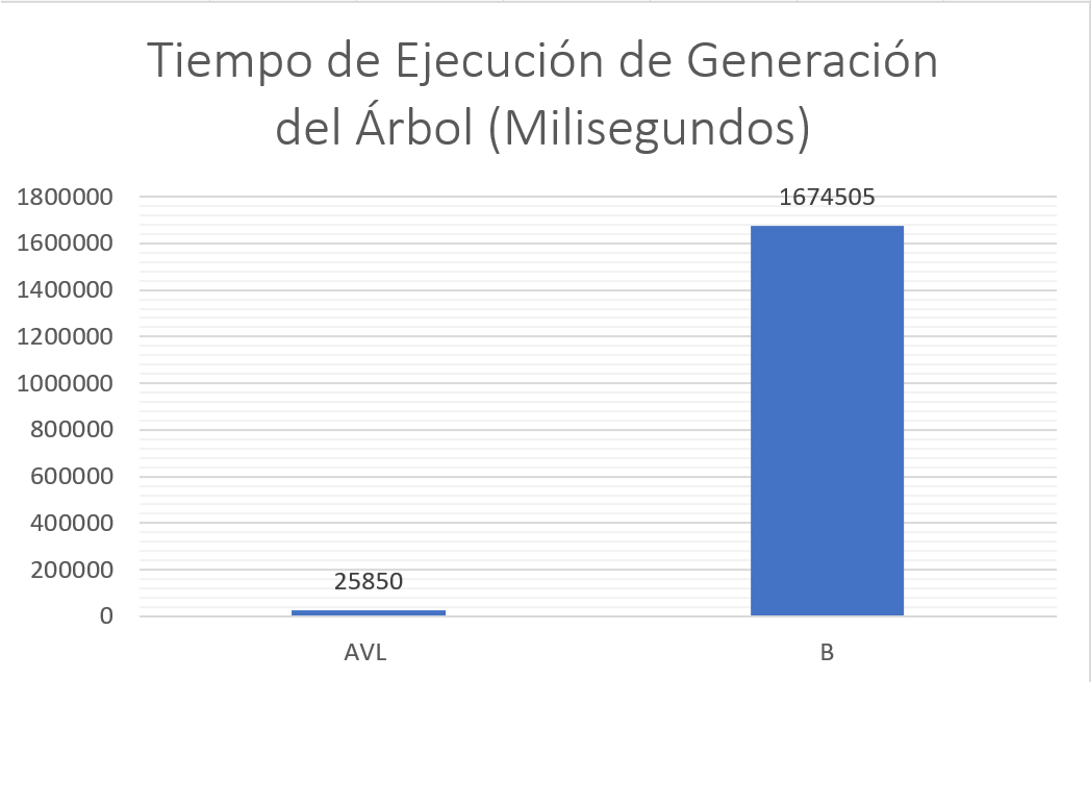
\includegraphics[angle=0,scale=0.6]{2000000.1 elem.png}
  
\end{figure}
\begin{figure}[ht]
  \centering
  \caption{Gráfica Comparativa del Tiempo en la Búsqueda de 10 números en el Árbol de 2000000 elementos}

  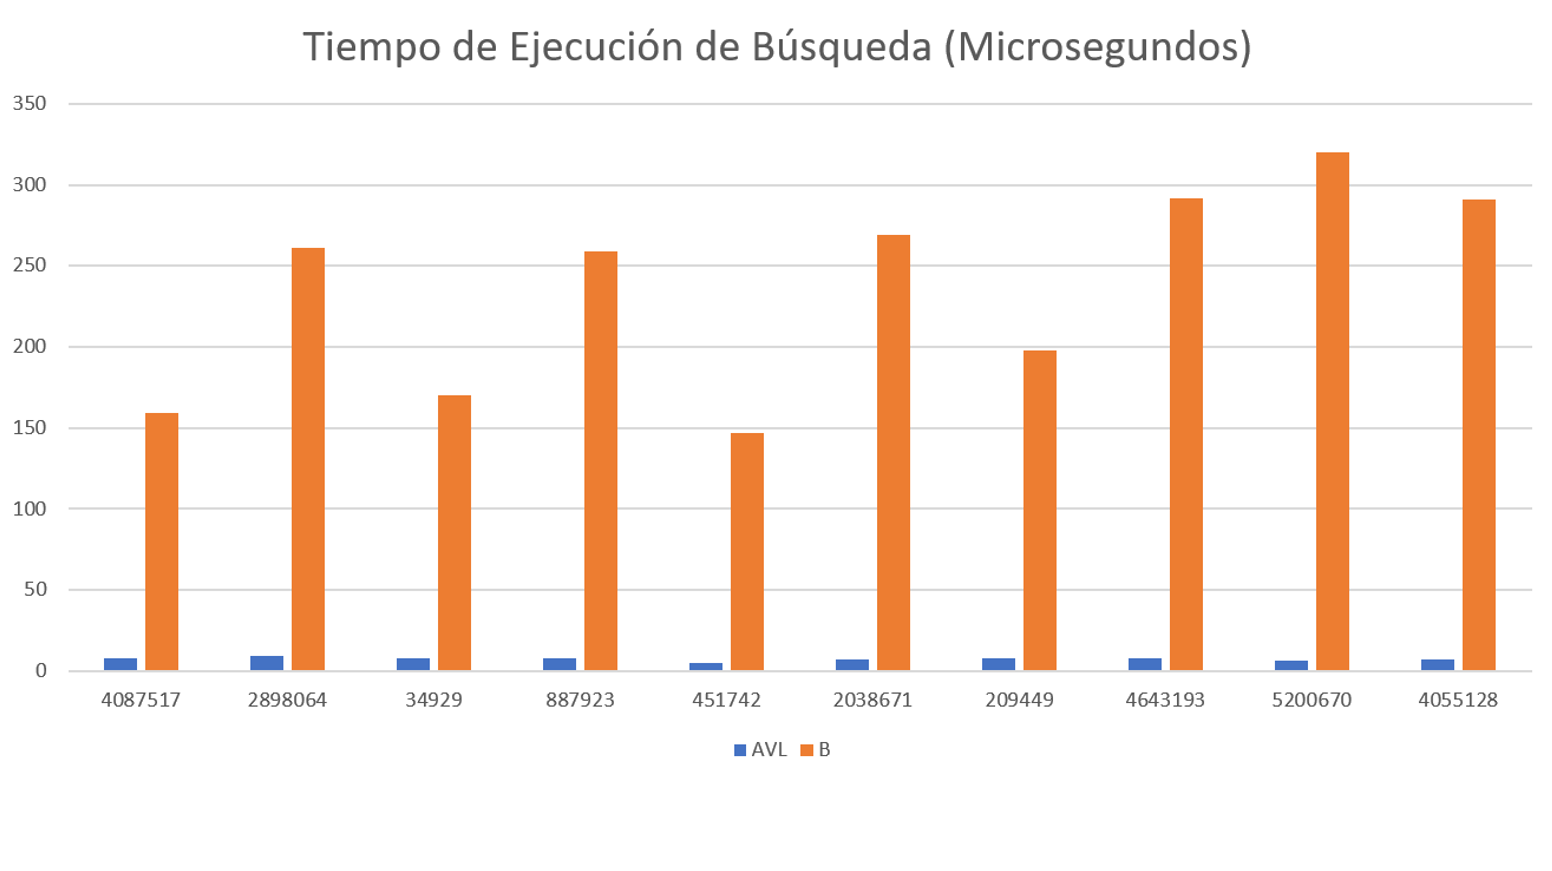
\includegraphics[angle=0,scale=0.53]{2000000.2 elem.png}
  
\end{figure}

\begin{figure}[ht]
  \centering
  \caption{Gráfica Comparativa del Tiempo en la Eliminación de 10 números en el Árbol de 2000000 elementos}

  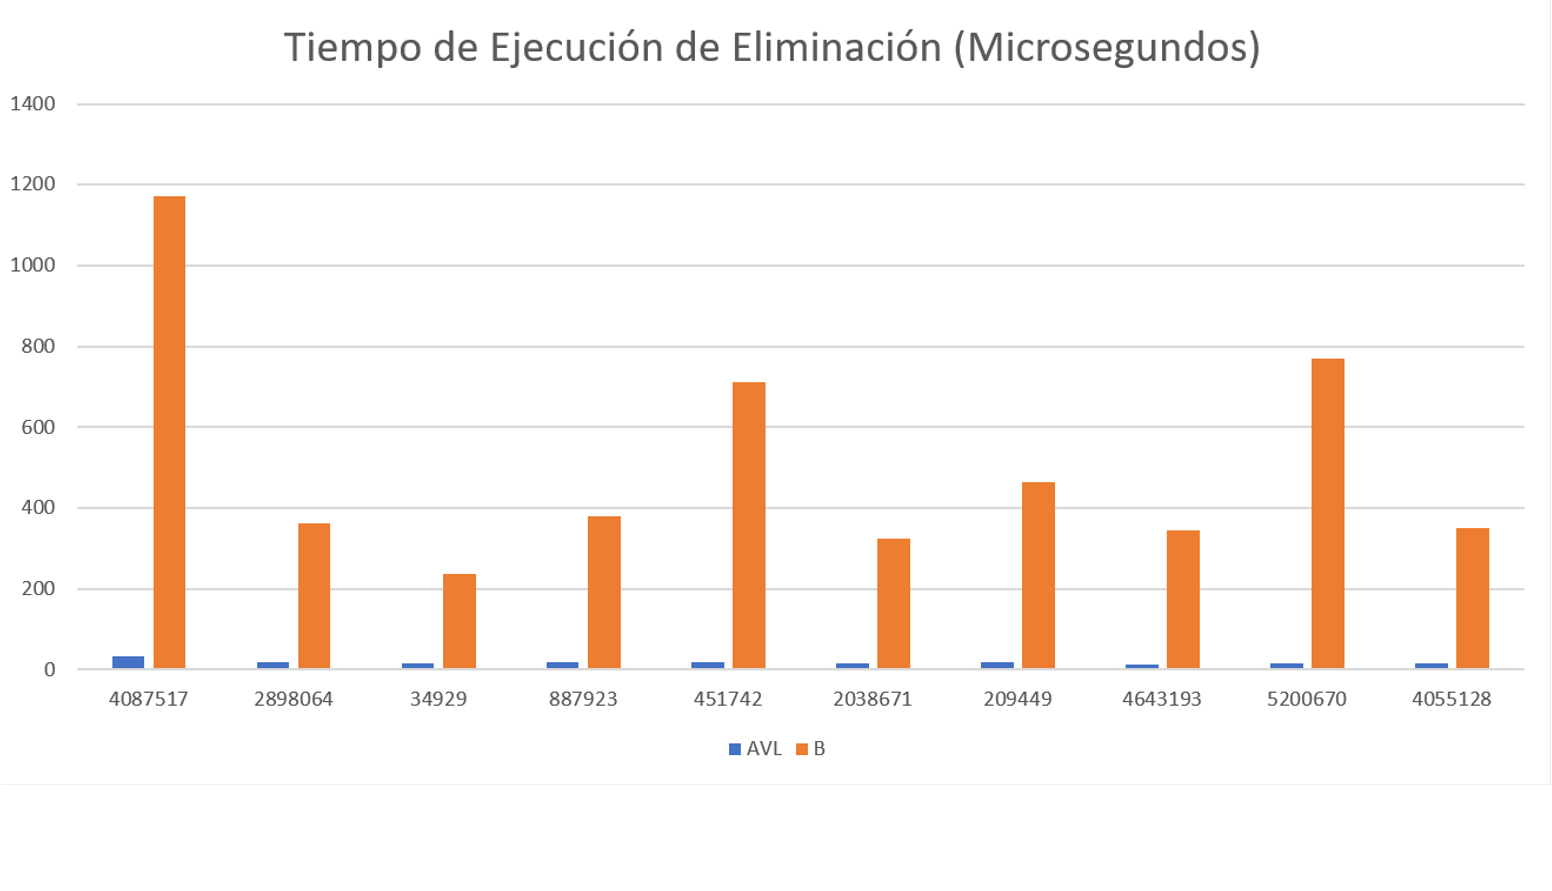
\includegraphics[angle=0,scale=0.5]{2000000.3 elem.png}
  
\end{figure}

\clearpage

%%--------------------------------------------
\section{Conclusiones}
Una vez hechas las pruebas y analizando los resultados que se obtuvieron, se puede apreciar que de las funciones que se implementaron, la inserción de elementos tiene un coste mayor de tiempo en ambos casos. Esto debido a la naturaleza de la función, de recorrer los elementos del árbol para ubicar su posición, así como las modificaciones que se deben hacer en caso de desbalance dentro del AVL o llenado de un nodo en el B.\\
La función que sigue en orden de coste de tiempo es la eliminación, ya que tiene que hacer una búsqueda del elemento para eliminarlo y hacer el o los reacomodos necesarios para que el árbol siga cumpliendo sus propiedades respectivas.
Al final, la búsqueda resulta ser la función que tiene menor coste, ya que solo necesita comparar ciertos valores para identificar si existe o no dentro del árbol.\\
Tal y como se puede ver en las gráficas, en ningún caso el árbol B resulta ser más eficiente que el AVL en cuestión temporal. Esto era de esperarse, ya que como se mencionó anteriormente, el B consume más tiempo abriendo, leyendo, escribiendo y cerrando archivos. Comparado con el AVL el cual solo tiene que acceder a la información en memoria RAM que es más rápida, por medio de los apuntadores.\\
Temporalmente hablando, el árbol AVL es más eficiente que el B, sin embargo no quiere decir que en todos los casos será así, ya que se tiene que considerar que el árbol AVL sólo servirá si el programa está corriendo, por lo que si se finaliza, los datos se perderán. Situación que no sucede en el B, ya que gracias a que se toma más tiempo escribiendo en ficheros, tiene la propiedad de que se puede hacer cualquier función ya mencionada aún reiniciando el programa. Esto sin tomar en cuenta que no hará tanto consumo de la memoria RAM, la cual suele ser bastante limitada, sobretodo si se está utilizando una Raspberry Pi, como fue en este caso.


\begin{thebibliography}{9}
\bibitem{cstdio} 
cplusplus.com. 2020. \textit{<cstdio> (stdio.h) }. Obtenido de:
\texttt{http://www.cplusplus.com/reference/cstdio/}


\bibitem{AVL} 
Rodewad, A.. 2012. \textit{AVL Tree | Set 2 (Deletion).} Geeks for Geeks. Obtenido de:
\\\texttt{http://www-cs-faculty.stanford.edu/\~{}uno/abcde.html}

\bibitem{B-Tree} 
Balasubramanian, N.. 2019 \textit{Delete Operation in B-Tree.} Geeks for Geeks. Obtenido de:
\\\texttt{http://www-cs-faculty.stanford.edu/\~{}uno/abcde.html}


\bibitem{Cubells_B} 
Cubells, V. (2020). “Árboles B” [Power Point] (Presentación de Clase).
\bibitem{Cubells_Bin} 
Cubells, V. (2020). “Árboles binarios de búsqueda” [Power Point] (Presentación de Clase).

\end{thebibliography}



\section{Información Acerca de las Referencias}
En varias ocasiones se acudió a las implementaciones publicadas por Geeks for Geeks para la realización de ambos árboles, la lógica que se sigue en cada una de las clases se encuentra muy apegada a la establecida por ellos. Por último, para la implementación del Árbol B en el disco, se utilizó la API publicada por cplusplus.com con respecto a su librería stdio.h, cuyos métodos resultaron ser muy útiles para escribir, leer y desplazarse por un archivo de tipo .bin y lograr almacenar la información de los nodos en el disco como resultado.
\fancyfoot[R]{Análisis de Algoritmos, Feb-Jun 2020}

\end{document}
\endinput